% =====================================================================
%  VibeBench -- architecture and methodology diagrams
%  Self-contained: compiles on its own (pdfLaTeX) in Overleaf.
%  To reuse a single figure in the thesis, copy the tikzpicture and the
%  style block in the preamble; no figure depends on another.
%
%  LAYOUT RULES OBSERVED HERE (do not break them when editing):
%   * text width is 16.6cm (a4paper, margin=2.2cm). Every picture is
%     built inside a \resizebox guarded to \textwidth, so a node added
%     later can never push a figure off the page.
%   * annotation notes are anchored explicitly (anchor=north/west/...)
%     and given a text width, so they wrap instead of overprinting.
%   * no note is placed with a negative offset onto another node.
% =====================================================================
\documentclass[11pt]{article}

\usepackage[a4paper,margin=2.2cm]{geometry}
\usepackage{tikz}
\usepackage{pgfplots}
\pgfplotsset{compat=1.18}
\usepackage{amsmath}
\usepackage{booktabs}
\usepackage{caption}
\usepackage{microtype}
\usepackage{amssymb}
\usepackage{pifont}

\usetikzlibrary{
  positioning, arrows.meta, shapes.geometric, shapes.multipart,
  calc, fit, backgrounds, decorations.pathreplacing, patterns
}

\captionsetup{font=small, labelfont=bf, width=0.95\textwidth}

% ---------------------------------------------------------------------
%  Shared visual language. One palette, one set of shapes, so the
%  figures read as a single system rather than unrelated drawings.
% ---------------------------------------------------------------------
\definecolor{vbInk}    {HTML}{1F2328}   % text / rules
\definecolor{vbStage}  {HTML}{2C5F7C}   % pipeline stages
\definecolor{vbStageBg}{HTML}{E8F0F5}
\definecolor{vbStore}  {HTML}{6B5B95}   % persisted artefacts
\definecolor{vbStoreBg}{HTML}{EFEAF5}
\definecolor{vbGood}   {HTML}{3B6B4A}   % kept / valid
\definecolor{vbGoodBg} {HTML}{E4EDE6}
\definecolor{vbDrop}   {HTML}{8B3A3A}   % excluded / failed
\definecolor{vbDropBg} {HTML}{F2E3E3}
\definecolor{vbWarn}   {HTML}{8A6D1F}   % caveats
\definecolor{vbWarnBg} {HTML}{F5EFDD}
\definecolor{vbNote}   {HTML}{6E6A63}   % annotations

\tikzset{
  font=\sffamily\small,
  stage/.style     ={rectangle, rounded corners=2pt, draw=vbStage, thick,
                     fill=vbStageBg, text=vbInk, align=center,
                     minimum height=11mm, inner xsep=3mm},
  store/.style     ={cylinder, shape border rotate=90, aspect=0.22,
                     draw=vbStore, thick, fill=vbStoreBg, text=vbInk,
                     align=center, minimum height=9mm, inner xsep=2mm},
  decision/.style  ={diamond, aspect=2.4, draw=vbStage, thick,
                     fill=vbStageBg, align=center, inner sep=1pt,
                     font=\sffamily\scriptsize},
  keep/.style      ={rectangle, rounded corners=2pt, draw=vbGood, thick,
                     fill=vbGoodBg, align=center, minimum height=10mm,
                     inner xsep=3mm},
  drop/.style      ={rectangle, rounded corners=2pt, draw=vbDrop, thick,
                     fill=vbDropBg, align=center, minimum height=8mm,
                     font=\sffamily\scriptsize, inner xsep=2mm},
  warn/.style      ={rectangle, rounded corners=2pt, draw=vbWarn, thick,
                     fill=vbWarnBg, align=left,
                     font=\sffamily\scriptsize, inner sep=2mm},
  commit/.style    ={circle, draw=vbInk, thick, fill=white,
                     minimum size=6mm, inner sep=0pt,
                     font=\sffamily\scriptsize},
  prcommit/.style  ={commit, fill=vbStageBg, draw=vbStage},
  flow/.style      ={-{Stealth[length=2.2mm]}, thick, draw=vbInk},
  thin flow/.style ={-{Stealth[length=1.8mm]}, semithick, draw=vbNote},
  dashflow/.style  ={-{Stealth[length=2.2mm]}, thick, draw=vbStore, dashed},
  note/.style      ={text=vbNote, font=\sffamily\scriptsize, align=left},
  lbl/.style       ={font=\sffamily\scriptsize, text=vbNote,
                     inner sep=1pt, fill=white, fill opacity=0.85,
                     text opacity=1},
  code/.style      ={font=\ttfamily\scriptsize},
  % ---- worked-example figure styles (SRP/DIP/OCP/LSP/ISP) --------------
  panel/.style   ={rectangle, rounded corners=3pt, draw=vbNote!45, thick,
                   fill=white, align=left, inner sep=3mm},
  srcpanel/.style={panel, draw=vbStage!55, fill=vbStageBg!30},
  calcpanel/.style={panel, draw=vbStore!55, fill=vbStoreBg!35},
  outpanel/.style={panel, draw=vbGood!65, fill=vbGoodBg!45},
  badge/.style   ={circle, draw=vbInk, fill=vbInk, text=white,
                   font=\sffamily\bfseries\scriptsize, inner sep=0pt,
                   minimum size=4.6mm},
  ptitle/.style  ={font=\sffamily\bfseries\scriptsize, text=vbInk, inner sep=0pt},
  astn/.style    ={rectangle, rounded corners=1.5pt, draw=vbStage, thick,
                   fill=white, font=\ttfamily\tiny, inner sep=1.4pt,
                   minimum height=3.6mm},
  astleaf/.style ={astn, draw=vbStore, fill=vbStoreBg!60},
  cellon/.style  ={rectangle, minimum size=5mm, draw=vbStage!45,
                   fill=vbStage!65, inner sep=0pt},
  celloff/.style ={rectangle, minimum size=5mm, draw=vbNote!30,
                   fill=white, inner sep=0pt},
  wetag/.style   ={font=\sffamily\scriptsize\itshape, text=vbInk,
                   fill=white, inner sep=1.2pt},
  verdict/.style ={rectangle, rounded corners=2pt, draw=vbDrop, very thick,
                   fill=vbDropBg, font=\sffamily\bfseries\small, text=vbDrop,
                   inner sep=2.2mm},
  okverdict/.style={rectangle, rounded corners=2pt, draw=vbGood, very thick,
                   fill=vbGoodBg, font=\sffamily\bfseries\small, text=vbGood,
                   inner sep=2.2mm},
  mod/.style     ={circle, draw=vbStage, very thick, fill=white,
                   font=\ttfamily\tiny, inner sep=0.6pt, minimum size=8.5mm},
  modnew/.style  ={mod, draw=vbDrop, fill=vbDropBg},
  imp/.style     ={-{Stealth[length=2mm]}, semithick, draw=vbNote},
  impnew/.style  ={-{Stealth[length=2.4mm]}, very thick, draw=vbDrop},
  brc/.style     ={rectangle, rounded corners=1.5pt, draw=vbStage, thick,
                   fill=vbStageBg!60, font=\ttfamily\tiny, inner sep=1.6pt,
                   minimum width=17mm},
  cls/.style     ={rectangle, draw=vbStage, very thick, fill=white,
                   align=left, inner sep=0pt, minimum width=46mm},
  clshdr/.style  ={rectangle, draw=vbStage, very thick, fill=vbStageBg,
                   font=\sffamily\bfseries\scriptsize, minimum width=46mm,
                   minimum height=6mm, inner sep=1pt},
  clsbody/.style ={rectangle, draw=vbStage, thick, fill=white,
                   font=\ttfamily\scriptsize, align=left, minimum width=46mm,
                   inner sep=2mm, text width=42mm},
  inherit/.style ={-{Triangle[open, length=3mm, width=3mm]}, very thick, draw=vbStage},
  impl/.style    ={rectangle, minimum size=5.4mm, draw=vbGood!55, fill=vbGood!45,
                   inner sep=0pt, font=\sffamily\tiny, text=white},
  stub/.style    ={rectangle, minimum size=5.4mm, draw=vbDrop!65, fill=vbDropBg,
                   inner sep=0pt, font=\sffamily\bfseries\tiny, text=vbDrop},
}

% Guard: never let a picture exceed the text block.
\newcommand{\fitpic}[1]{\resizebox{\ifdim\width>\textwidth\textwidth\else\width\fi}{!}{#1}}
% badge + title placed above a panel's top-left corner
\newcommand{\steptitle}[3]{%
  \node[badge, anchor=south west] at ($(#1.north west)+(0.05,0.16)$) (#1bdg) {#2};
  \node[ptitle, anchor=west] at ($(#1bdg.east)+(0.10,0)$) {#3};}

\begin{document}

\begin{center}
{\Large\bfseries\sffamily VibeBench --- architecture and method}\\[2mm]
{\sffamily\small Measuring SOLID conformance of autonomous coding agents on real merged pull requests}
\end{center}
\vspace{2mm}

% =====================================================================
\section*{1. End-to-end pipeline (engineering view)}
% =====================================================================

\begin{figure}[h]
\centering
\fitpic{%
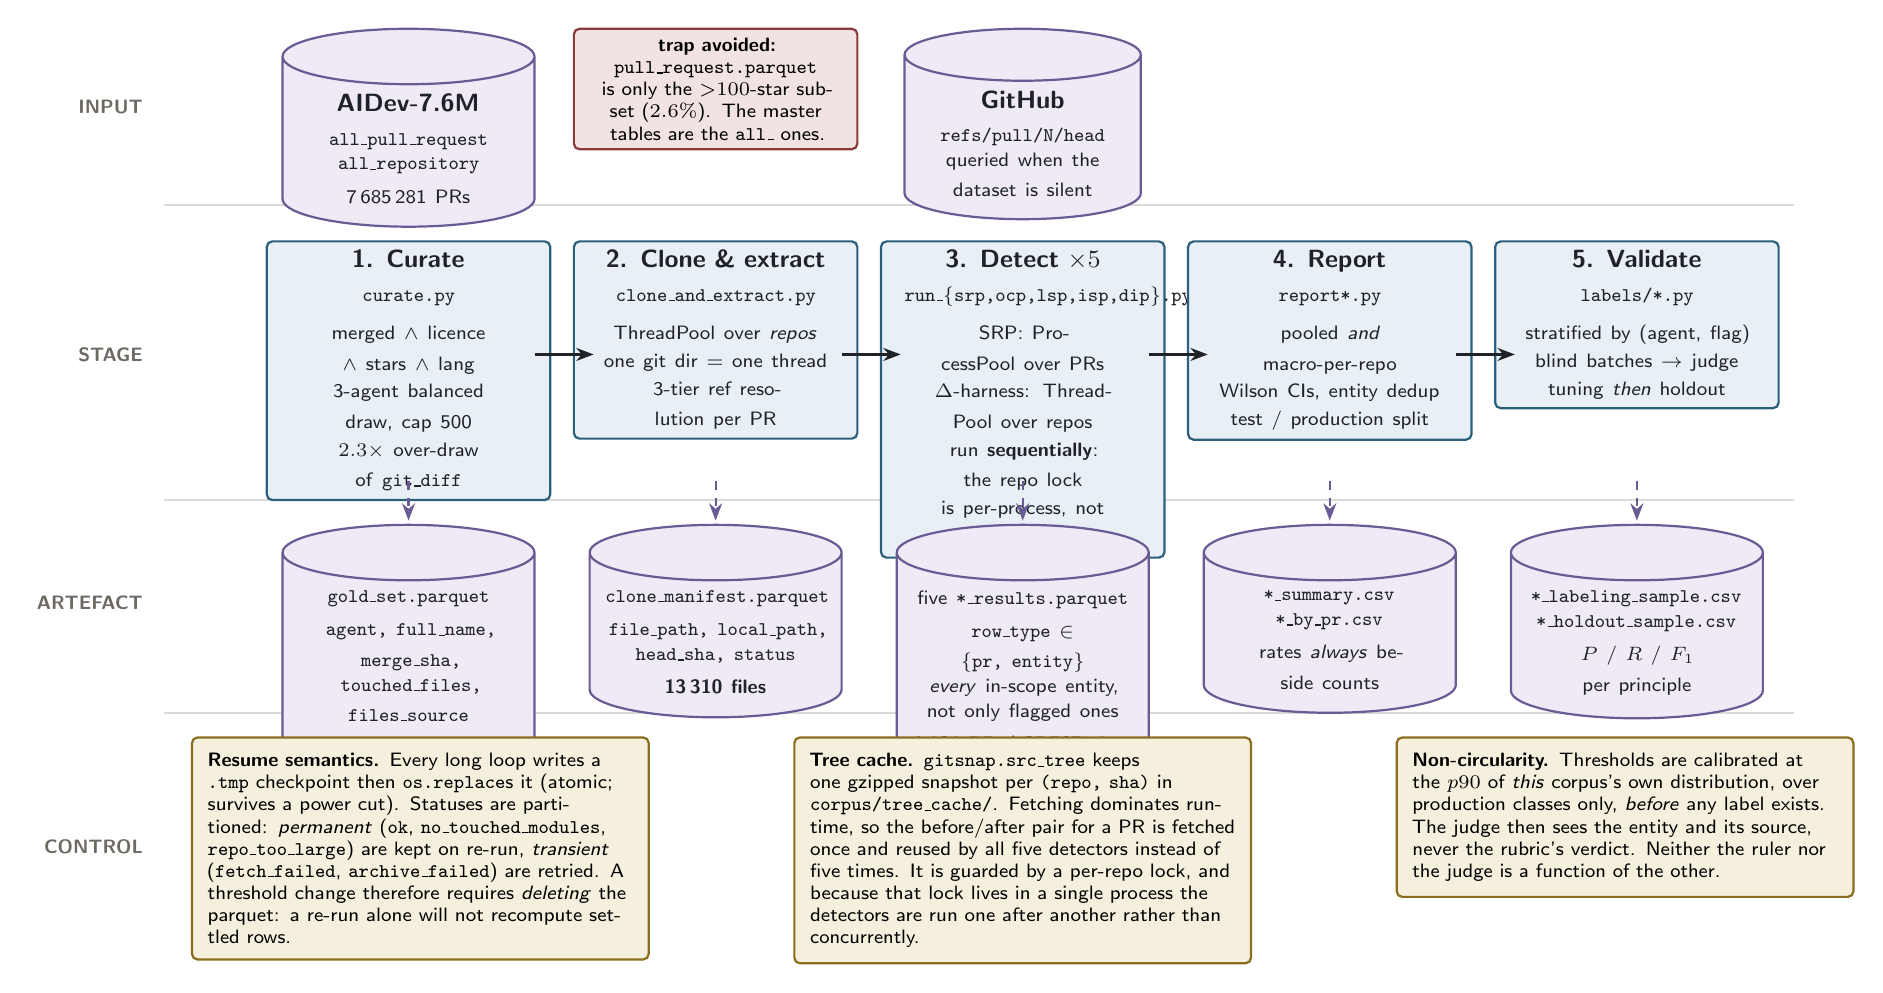
\begin{tikzpicture}[node distance=0mm]

% Row anchors (anchor=north => value is the TOP edge of that row's boxes).
% Chosen with clearance for the tallest box in each row; dividers sit in the gaps.
%   INPUT     top  0.70   bottom ~ -1.20
%   STAGE     top -2.00   bottom ~ -5.05
%   ARTEFACT  top -5.60   bottom ~ -7.75
%   CONTROL   top -8.30   bottom ~ -11.6

\foreach \y in {-1.55,-5.30,-8.00} \draw[vbNote!25, semithick] (-2.2,\y) -- (18.5,\y);

\node[font=\sffamily\bfseries\scriptsize, text=vbNote, anchor=east] at (-2.35,-0.30) {INPUT};
\node[font=\sffamily\bfseries\scriptsize, text=vbNote, anchor=east] at (-2.35,-3.45) {STAGE};
\node[font=\sffamily\bfseries\scriptsize, text=vbNote, anchor=east] at (-2.35,-6.60) {ARTEFACT};
\node[font=\sffamily\bfseries\scriptsize, text=vbNote, anchor=east] at (-2.35,-9.70) {CONTROL};

% ============ INPUT lane ============
\node[store, text width=28mm, anchor=north] at (0.9,0.70)
  {\textbf{AIDev-7.6M}\\[1pt]
   {\scriptsize\ttfamily all\_pull\_request}\\[-2pt]{\scriptsize\ttfamily all\_repository}\\[1pt]
   {\scriptsize 7\,685\,281 PRs}};
\node[drop, text width=32mm, anchor=north] at (4.8,0.70)
  {\textbf{trap avoided:} \texttt{pull\_request.parquet} is only the ${>}100$-star subset
   ($2.6\%$). The master tables are the \texttt{all\_} ones.};
\node[store, text width=26mm, anchor=north] at (8.7,0.70)
  {\textbf{GitHub}\\[1pt]{\scriptsize\ttfamily refs/pull/N/head}\\[-2pt]
   {\scriptsize queried when the dataset is silent}};

% ============ STAGE lane ============
\node[stage, text width=30mm, anchor=north] at (0.9,-2.00)
  {\textbf{1. Curate}\\[1pt]{\scriptsize\ttfamily curate.py}\\[3pt]
   {\scriptsize merged $\wedge$ licence $\wedge$ stars $\wedge$ lang}\\[-1pt]
   {\scriptsize 3-agent balanced draw, cap 500}\\[-1pt]
   {\scriptsize $2.3\times$ over-draw of \texttt{git\_diff}}};

\node[stage, text width=30mm, anchor=north] at (4.8,-2.00)
  {\textbf{2. Clone \& extract}\\[1pt]{\scriptsize\ttfamily clone\_and\_extract.py}\\[3pt]
   {\scriptsize ThreadPool over \emph{repos}}\\[-1pt]
   {\scriptsize one git dir $=$ one thread}\\[-1pt]
   {\scriptsize 3-tier ref resolution per PR}};

\node[stage, text width=30mm, anchor=north] at (8.7,-2.00)
  {\textbf{3. Detect} $\times5$\\[1pt]{\scriptsize\ttfamily run\_\{srp,ocp,lsp,isp,dip\}.py}\\[3pt]
   {\scriptsize SRP: ProcessPool over PRs}\\[-1pt]
   {\scriptsize $\Delta$-harness: ThreadPool over repos}\\[-1pt]
   {\scriptsize run \textbf{sequentially}: the repo lock}\\[-1pt]
   {\scriptsize is per-process, not cross-process}};

\node[stage, text width=30mm, anchor=north] at (12.6,-2.00)
  {\textbf{4. Report}\\[1pt]{\scriptsize\ttfamily report*.py}\\[3pt]
   {\scriptsize pooled \emph{and} macro-per-repo}\\[-1pt]
   {\scriptsize Wilson CIs, entity dedup}\\[-1pt]
   {\scriptsize test / production split}};

\node[stage, text width=30mm, anchor=north] at (16.5,-2.00)
  {\textbf{5. Validate}\\[1pt]{\scriptsize\ttfamily labels/*.py}\\[3pt]
   {\scriptsize stratified by (agent, flag)}\\[-1pt]
   {\scriptsize blind batches $\to$ judge}\\[-1pt]
   {\scriptsize tuning \emph{then} holdout}};

\foreach \x in {2.5,6.4,10.3,14.2}
  \draw[flow] (\x,-3.45) -- (\x+0.75,-3.45);

% ============ ARTEFACT lane ============
\node[store, text width=28mm, anchor=north] at (0.9,-5.60)
  {{\scriptsize\ttfamily gold\_set.parquet}\\[1pt]
   {\scriptsize\ttfamily agent, full\_name, merge\_sha,}\\[-2pt]
   {\scriptsize\ttfamily touched\_files, files\_source}\\[1pt]{\scriptsize\textbf{1\,786 rows}}};
\node[store, text width=28mm, anchor=north] at (4.8,-5.60)
  {{\scriptsize\ttfamily clone\_manifest.parquet}\\[1pt]
   {\scriptsize\ttfamily file\_path, local\_path,}\\[-2pt]
   {\scriptsize\ttfamily head\_sha, status}\\[1pt]{\scriptsize\textbf{13\,310 files}}};
\node[store, text width=28mm, anchor=north] at (8.7,-5.60)
  {{\scriptsize five \ttfamily *\_results.parquet}\\[1pt]
   {\scriptsize\ttfamily row\_type $\in$ \{pr, entity\}}\\[-2pt]
   {\scriptsize \emph{every} in-scope entity,}\\[-2pt]
   {\scriptsize not only flagged ones}\\[1pt]{\scriptsize\textbf{1\,464 PR / 35\,767 class}}};
\node[store, text width=28mm, anchor=north] at (12.6,-5.60)
  {{\scriptsize\ttfamily *\_summary.csv}\\[-2pt]{\scriptsize\ttfamily *\_by\_pr.csv}\\[1pt]
   {\scriptsize rates \emph{always} beside counts}};
\node[store, text width=28mm, anchor=north] at (16.5,-5.60)
  {{\scriptsize\ttfamily *\_labeling\_sample.csv}\\[-2pt]{\scriptsize\ttfamily *\_holdout\_sample.csv}\\[1pt]
   {\scriptsize $P$ / $R$ / $F_1$ per principle}};

\foreach \x in {0.9,4.8,8.7,12.6,16.5}
  \draw[dashflow] (\x,-5.06) -- (\x,-5.56);

% ============ CONTROL lane ============
\node[warn, text width=54mm, anchor=north] at (1.05,-8.30)
  {\textbf{Resume semantics.} Every long loop writes a \texttt{.tmp} checkpoint then
   \texttt{os.replace}s it (atomic; survives a power cut). Statuses are partitioned:
   \emph{permanent} (\texttt{ok}, \texttt{no\_touched\_modules}, \texttt{repo\_too\_large})
   are kept on re-run, \emph{transient} (\texttt{fetch\_failed}, \texttt{archive\_failed})
   are retried. A threshold change therefore requires \emph{deleting} the parquet: a re-run
   alone will not recompute settled rows.};

\node[warn, text width=54mm, anchor=north] at (8.70,-8.30)
  {\textbf{Tree cache.} \texttt{gitsnap.src\_tree} keeps one gzipped snapshot per
   \texttt{(repo, sha)} in \texttt{corpus/tree\_cache/}. Fetching dominates runtime, so the
   before/after pair for a PR is fetched once and reused by all five detectors instead of
   five times. It is guarded by a per-repo lock, and because that lock lives in a single
   process the detectors are run one after another rather than concurrently.};

\node[warn, text width=54mm, anchor=north] at (16.35,-8.30)
  {\textbf{Non-circularity.} Thresholds are calibrated at the $p90$ of \emph{this} corpus's
   own distribution, over production classes only, \emph{before} any label exists. The judge
   then sees the entity and its source, never the rubric's verdict. Neither the ruler nor the
   judge is a function of the other.};

\end{tikzpicture}}
\caption{\textbf{End-to-end pipeline, engineering view.} Read top to bottom: what enters the
system, what transforms it, what is written to disk, and the invariants that hold across the
whole run. Each stage consumes only the previous stage's artefact, so any stage can be re-run
without rebuilding the ones before it. The three control blocks are what make a multi-day run
reproducible --- crash-safe resumption, a cache that makes the dominant cost payable once, and
an ordering that keeps threshold calibration independent of labelling.}
\end{figure}

\clearpage

% =====================================================================
\section*{2. Corpus selection}
% =====================================================================

\begin{figure}[h]
\centering
\fitpic{%
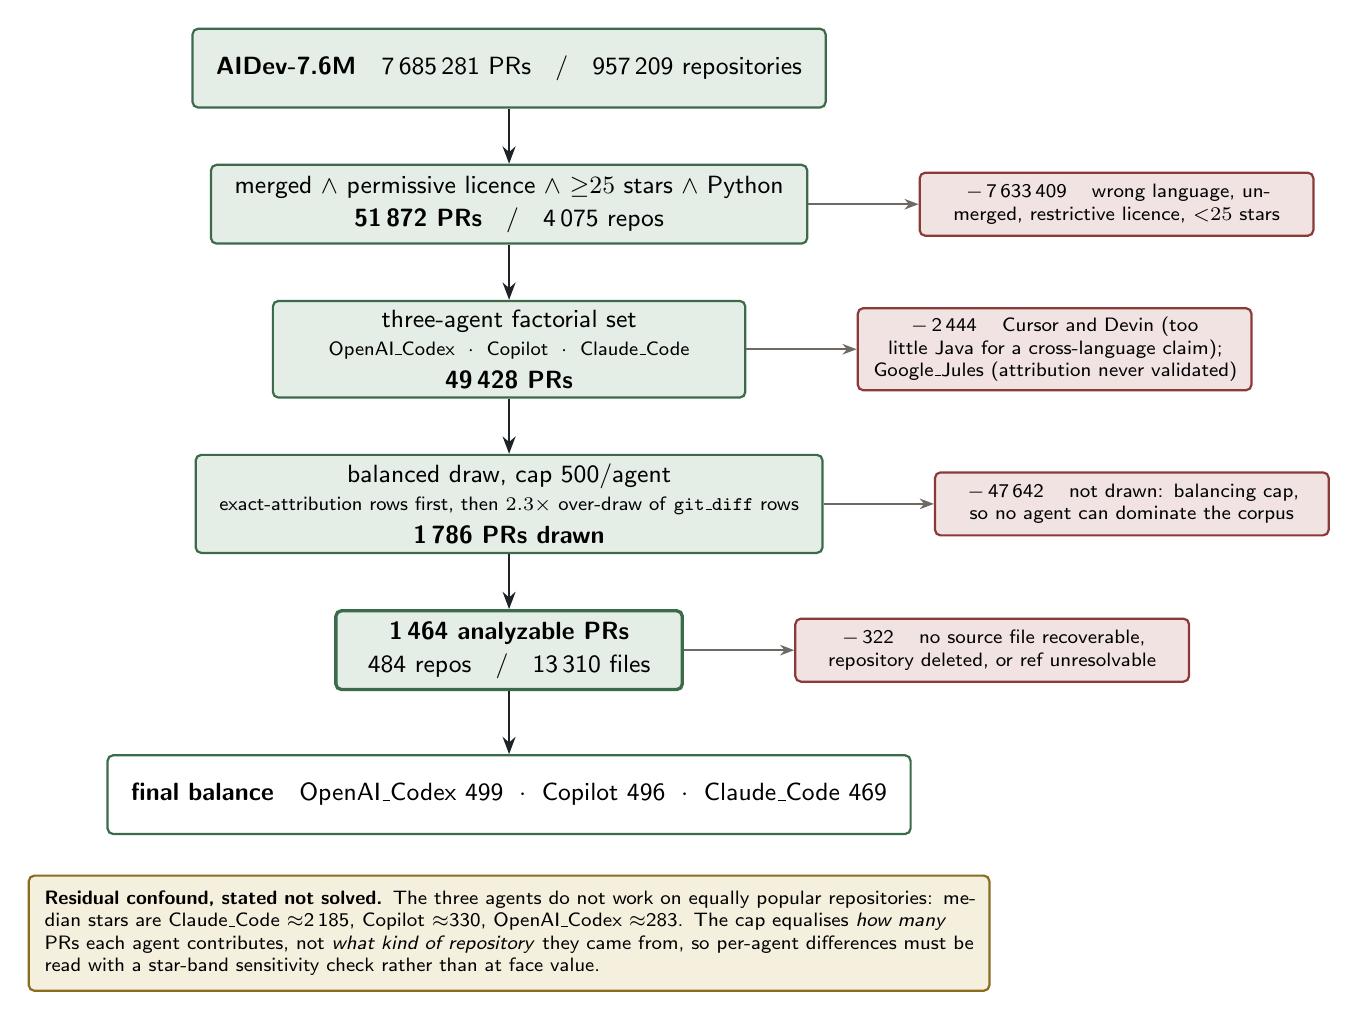
\begin{tikzpicture}[node distance=7mm]

\node[keep, minimum width=76mm] (n0)
  {\textbf{AIDev-7.6M}\quad 7\,685\,281 PRs \; / \; 957\,209 repositories};
\node[keep, below=of n0, minimum width=68mm] (n1)
  {merged $\wedge$ permissive licence $\wedge$ ${\geq}25$ stars $\wedge$ Python\\[1pt]\textbf{51\,872 PRs} \; / \; 4\,075 repos};
\node[keep, below=of n1, minimum width=60mm] (n2)
  {three-agent factorial set\\[-1pt]{\scriptsize OpenAI\_Codex \;$\cdot$\; Copilot \;$\cdot$\; Claude\_Code}\\[1pt]\textbf{49\,428 PRs}};
\node[keep, below=of n2, minimum width=52mm] (n3)
  {balanced draw, cap 500/agent\\[-1pt]{\scriptsize exact-attribution rows first, then $2.3\times$ over-draw of \texttt{git\_diff} rows}\\[1pt]\textbf{1\,786 PRs drawn}};
\node[keep, below=of n3, minimum width=44mm, draw=vbGood, very thick] (n4)
  {\textbf{1\,464 analyzable PRs}\\[1pt]484 repos \; / \; 13\,310 files};

\foreach \a/\b in {n0/n1, n1/n2, n2/n3, n3/n4} \draw[flow] (\a) -- (\b);

% exclusions on the right -- fixed width so they cannot collide
\node[drop, right=14mm of n1, text width=46mm] (d1)
  {$-$\,7\,633\,409 \;\; wrong language, unmerged, restrictive licence, ${<}25$ stars};
\node[drop, right=14mm of n2, text width=46mm] (d2)
  {$-$\,2\,444 \;\; Cursor and Devin (too little Java for a cross-language claim);
   Google\_Jules (attribution never validated)};
\node[drop, right=14mm of n3, text width=46mm] (d3)
  {$-$\,47\,642 \;\; not drawn: balancing cap, so no agent can dominate the corpus};
\node[drop, right=14mm of n4, text width=46mm] (d4)
  {$-$\,322 \;\; no source file recoverable, repository deleted, or ref unresolvable};

\foreach \a/\b in {n1/d1, n2/d2, n3/d3, n4/d4} \draw[thin flow] (\a) -- (\b);

\node[keep, below=8mm of n4, minimum width=76mm, fill=white] (bal)
  {\textbf{final balance}\quad OpenAI\_Codex 499 \;$\cdot$\; Copilot 496 \;$\cdot$\; Claude\_Code 469};
\draw[flow] (n4) -- (bal);

\node[warn, below=5mm of bal, anchor=north, text width=118mm]
  {\textbf{Residual confound, stated not solved.} The three agents do not work on equally
  popular repositories: median stars are Claude\_Code $\approx$2\,185, Copilot $\approx$330,
  OpenAI\_Codex $\approx$283. The cap equalises \emph{how many} PRs each agent contributes,
  not \emph{what kind of repository} they came from, so per-agent differences must be read
  with a star-band sensitivity check rather than at face value.};

\end{tikzpicture}}
\caption{\textbf{Corpus selection funnel.} Each stage reports what survives (left) and what is
removed and why (right), so the sample is reconstructible from the public dataset. The cap
equalises agent contribution: uncapped, one agent supplies most of the corpus and every
per-agent rate is dominated by that agent's own repository mix rather than by its behaviour.}
\end{figure}

\clearpage

% =====================================================================
\section*{3. What a ``tree'' is, and how a PR becomes a measurement}
% =====================================================================

\begin{figure}[h]
\centering
\fitpic{%
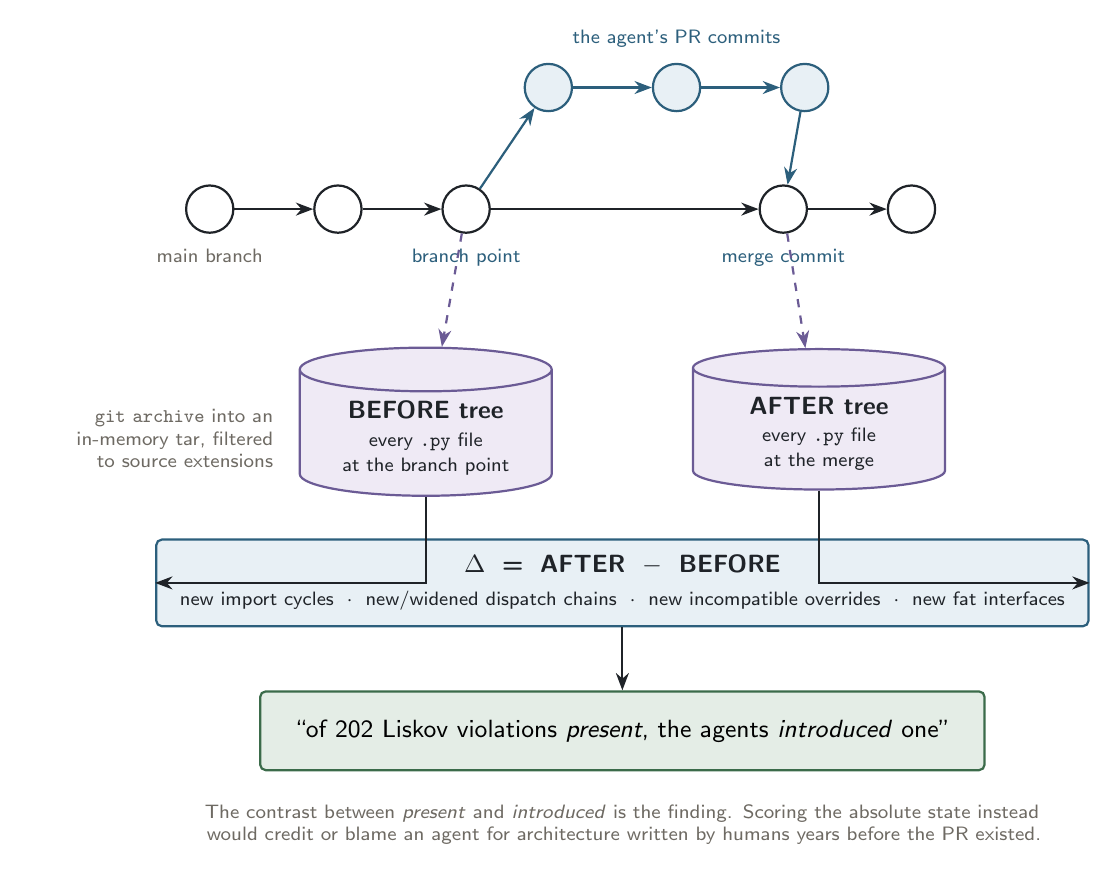
\begin{tikzpicture}[node distance=9mm]

% main branch
\node[commit] (b0) {};
\node[commit, right=10mm of b0] (b1) {};
\node[commit, right=10mm of b1] (base) {};
\node[commit, right=34mm of base] (m) {};
\node[commit, right=10mm of m] (b3) {};
\draw[flow] (b0)--(b1); \draw[flow] (b1)--(base);
\draw[flow] (base)--(m); \draw[flow] (m)--(b3);
\node[lbl, below=1.5mm of b0, anchor=north] {main branch};
\node[lbl, below=1.5mm of base, anchor=north, text=vbStage] {branch point};
\node[lbl, below=1.5mm of m, anchor=north, text=vbStage] {merge commit};

% PR branch
\node[prcommit, above right=11mm and 6mm of base] (p1) {};
\node[prcommit, right=10mm of p1] (p2) {};
\node[prcommit, right=10mm of p2] (p3) {};
\draw[flow, draw=vbStage] (base) -- (p1);
\draw[flow, draw=vbStage] (p1) -- (p2);
\draw[flow, draw=vbStage] (p2) -- (p3);
\draw[flow, draw=vbStage] (p3) -- (m);
\node[lbl, above=1.5mm of p2, anchor=south, text=vbStage] {the agent's PR commits};

% the two trees
\node[store, below left=16mm and -8mm of base, minimum width=32mm] (tb)
  {\textbf{BEFORE tree}\\[-1pt]{\scriptsize every \texttt{.py} file}\\[-2pt]{\scriptsize at the branch point}};
\node[store, below right=16mm and -8mm of m, minimum width=32mm] (ta)
  {\textbf{AFTER tree}\\[-1pt]{\scriptsize every \texttt{.py} file}\\[-2pt]{\scriptsize at the merge}};
\draw[dashflow] (base) -- (tb);
\draw[dashflow] (m) -- (ta);

\node[note, left=2mm of tb, anchor=east, text width=30mm, align=right]
  {\texttt{git archive} into an in-memory tar, filtered to source extensions};

% the delta
\node[stage, below=13mm of $(tb)!0.5!(ta)$, minimum width=92mm] (delta)
  {\textbf{$\Delta$ \;=\; AFTER \;$-$\; BEFORE}\\[1pt]
   {\scriptsize new import cycles \;$\cdot$\; new/widened dispatch chains \;$\cdot$\; new
    incompatible overrides \;$\cdot$\; new fat interfaces}};
\draw[flow] (tb) |- (delta.west);
\draw[flow] (ta) |- (delta.east);

\node[keep, below=8mm of delta, minimum width=92mm] (claim)
  {``of 202 Liskov violations \emph{present}, the agents \emph{introduced} one''};
\draw[flow] (delta) -- (claim);

\node[note, below=3mm of claim, anchor=north, text width=112mm, align=center]
  {The contrast between \emph{present} and \emph{introduced} is the finding. Scoring the
   absolute state instead would credit or blame an agent for architecture written by humans
   years before the PR existed.};

\end{tikzpicture}}
\caption{\textbf{The delta method.} A \emph{tree} is a snapshot of every source file at one
commit. Two are taken per pull request --- at its branch point and at its merge --- and the
principles are evaluated on the difference between them. The branch point is located with
\texttt{merge-base} against the default branch, \emph{not} as the merge commit's first parent:
for a multi-commit pull request the parent is the PR's own penultimate commit, which would
capture only its final commit and silently understate everything the agent wrote.}
\end{figure}

\clearpage

% =====================================================================
\section*{4. Resolving a pull request to a commit pair}
% =====================================================================

\begin{figure}[h]
\centering
\fitpic{%
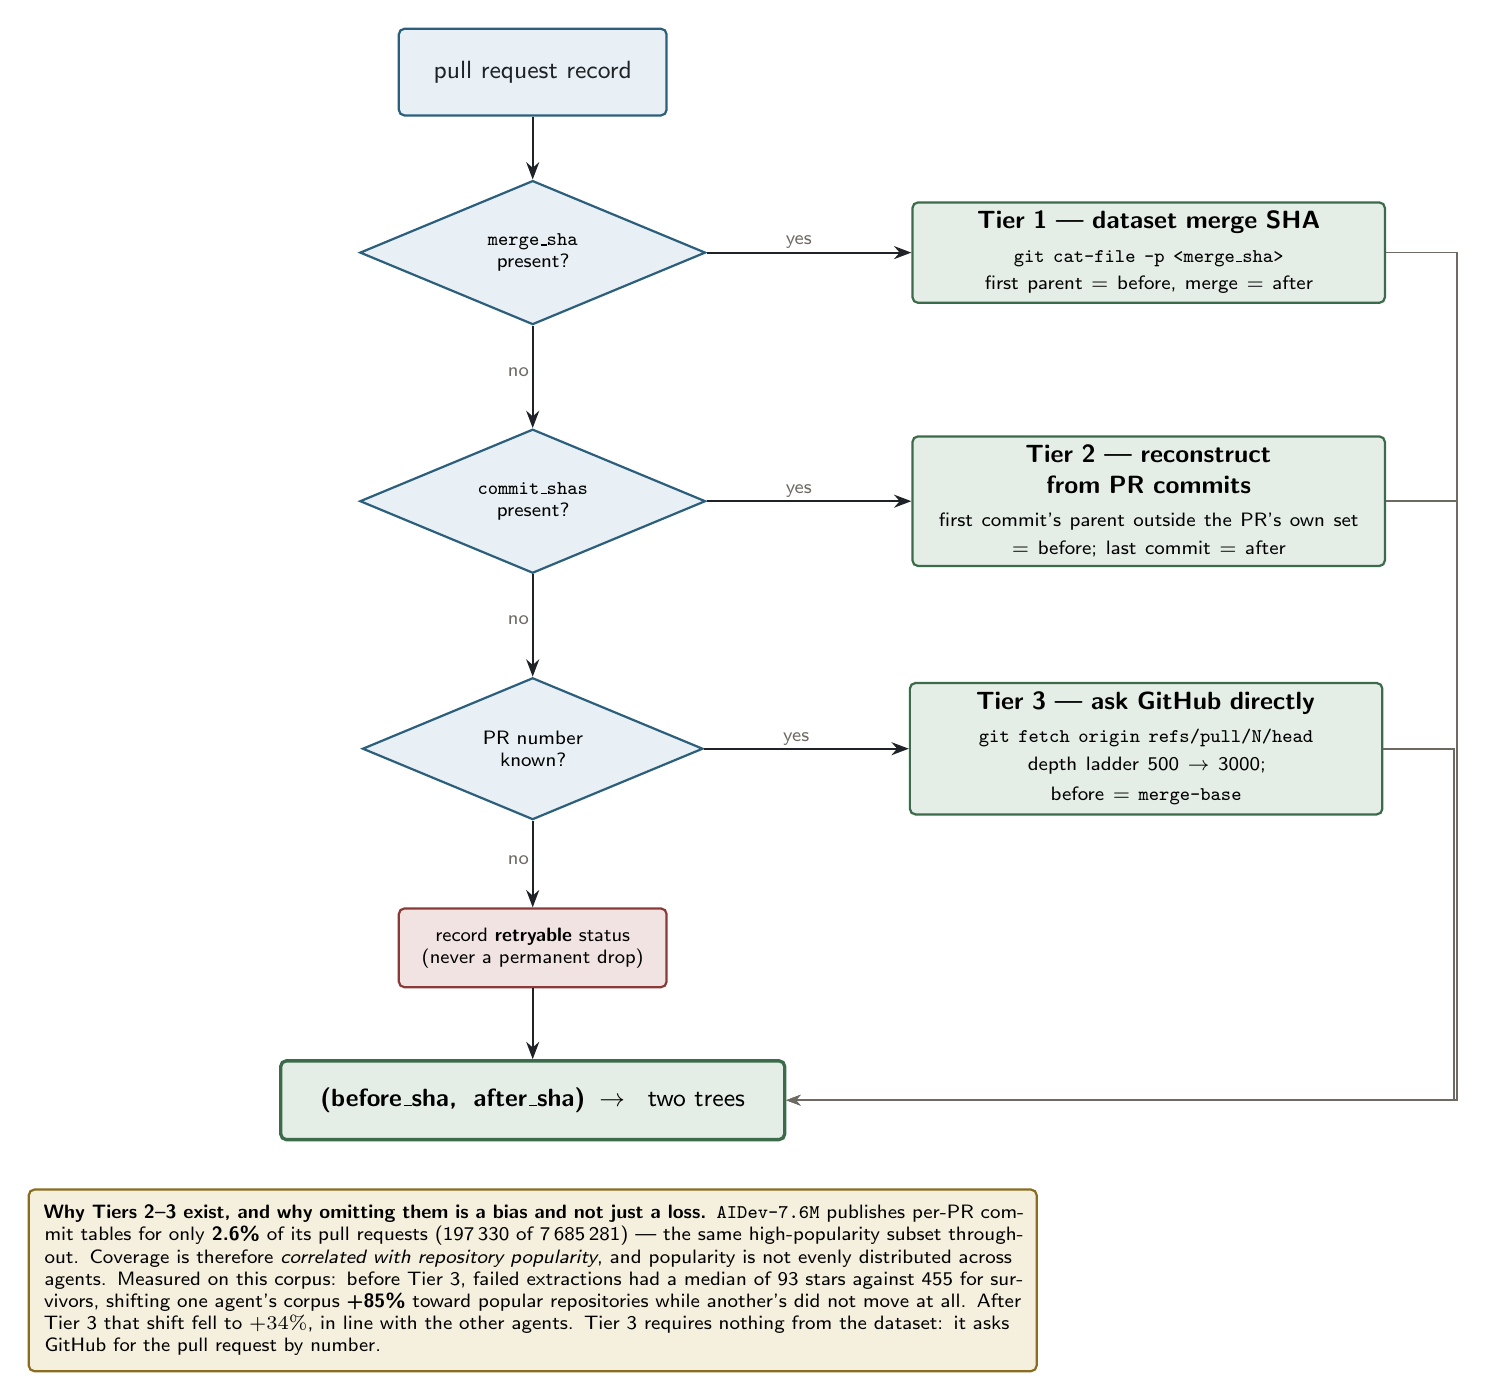
\begin{tikzpicture}[node distance=6mm]

% ---- vertical ladder: each tier is its own row (fits page width) ----
\node[stage, minimum width=34mm] (in) {pull request record};

\node[decision, below=8mm of in, text width=30mm] (d1)
  {\texttt{merge\_sha}\\present?};
\node[keep, right=26mm of d1, text width=54mm] (t1)
  {\textbf{Tier 1 --- dataset merge SHA}\\[1pt]
   {\scriptsize\ttfamily git cat-file -p <merge\_sha>}\\[-1pt]
   {\scriptsize first parent $=$ before, merge $=$ after}};

\node[decision, below=13mm of d1, text width=30mm] (d2)
  {\texttt{commit\_shas}\\present?};
\node[keep, right=26mm of d2, text width=54mm] (t2)
  {\textbf{Tier 2 --- reconstruct from PR commits}\\[1pt]
   {\scriptsize first commit's parent outside the PR's own set}\\[-1pt]
   {\scriptsize $=$ before; last commit $=$ after}};

\node[decision, below=13mm of d2, text width=30mm] (d3)
  {PR number\\known?};
\node[keep, right=26mm of d3, text width=54mm] (t3)
  {\textbf{Tier 3 --- ask GitHub directly}\\[1pt]
   {\scriptsize\ttfamily git fetch origin refs/pull/N/head}\\[-1pt]
   {\scriptsize depth ladder 500 $\to$ 3000; before $=$ \texttt{merge-base}}};

\node[drop, below=11mm of d3, minimum width=34mm, minimum height=10mm] (fail)
  {record \textbf{retryable} status\\{\scriptsize (never a permanent drop)}};

\draw[flow] (in) -- (d1);
\draw[flow] (d1) -- node[lbl, left, pos=0.45] {no} (d2);
\draw[flow] (d2) -- node[lbl, left, pos=0.45] {no} (d3);
\draw[flow] (d3) -- node[lbl, left, pos=0.45] {no} (fail);
\foreach \d/\t in {d1/t1, d2/t2, d3/t3}
  \draw[flow] (\d) -- node[lbl, above, pos=0.45] {yes} (\t);

% converge
\node[keep, below=9mm of fail, minimum width=64mm, draw=vbGood, very thick] (pair)
  {\textbf{(before\_sha,\; after\_sha)}\;\;$\to$\;\; two trees};
\foreach \t in {t1,t2,t3} \draw[thin flow] (\t.east) -- ++(9mm,0) |- (pair.east);
\draw[flow] (fail) -- (pair);

\node[warn, below=6mm of pair, anchor=north, text width=124mm]
  {\textbf{Why Tiers 2--3 exist, and why omitting them is a bias and not just a loss.}
   \texttt{AIDev-7.6M} publishes per-PR commit tables for only \textbf{2.6\%} of its pull
   requests (197\,330 of 7\,685\,281) --- the same high-popularity subset throughout. Coverage
   is therefore \emph{correlated with repository popularity}, and popularity is not evenly
   distributed across agents. Measured on this corpus: before Tier 3, failed extractions had a
   median of 93 stars against 455 for survivors, shifting one agent's corpus \textbf{+85\%}
   toward popular repositories while another's did not move at all. After Tier 3 that shift
   fell to $+34\%$, in line with the other agents. Tier 3 requires nothing from the dataset:
   it asks GitHub for the pull request by number.};

\end{tikzpicture}}
\caption{\textbf{Three-tier commit resolution.} The ladder is tried in order and stops at the
first tier that resolves. A pull request that reaches the bottom is recorded with a
\emph{retryable} status rather than discarded, so a transient network failure never silently
removes a PR from the corpus --- only a permanent status does, and those are enumerated.}
\end{figure}

\clearpage

% =====================================================================
\section*{5. Units of analysis}
% =====================================================================

\begin{figure}[h]
\centering
\fitpic{%
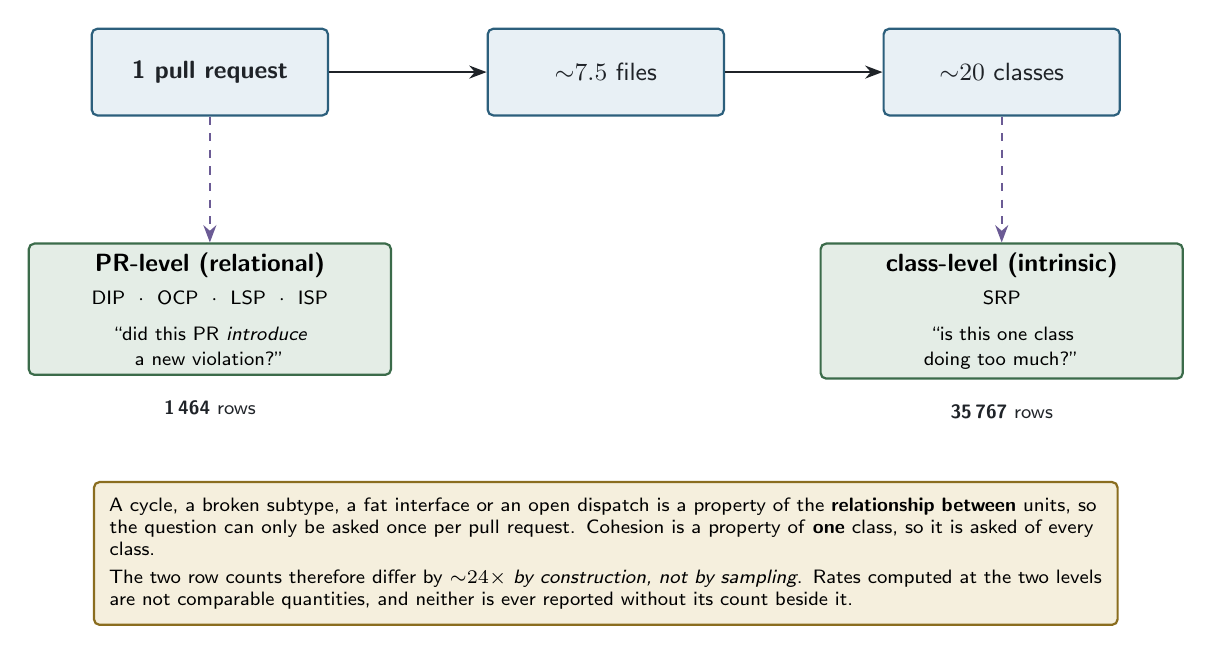
\begin{tikzpicture}[node distance=6mm]

\node[stage, minimum width=30mm] (pr) {\textbf{1 pull request}};
\node[stage, right=20mm of pr, minimum width=30mm] (file) {${\sim}7.5$ files};
\node[stage, right=20mm of file, minimum width=30mm] (cls) {${\sim}20$ classes};
\draw[flow] (pr) -- (file); \draw[flow] (file) -- (cls);

\node[keep, below=16mm of pr, minimum width=46mm] (prlevel)
  {\textbf{PR-level (relational)}\\[1pt]
   {\scriptsize DIP \;$\cdot$\; OCP \;$\cdot$\; LSP \;$\cdot$\; ISP}\\[2pt]
   {\scriptsize ``did this PR \emph{introduce}}\\[-2pt]
   {\scriptsize a new violation?''}};
\node[keep, below=16mm of cls, minimum width=46mm] (clslevel)
  {\textbf{class-level (intrinsic)}\\[1pt]
   {\scriptsize SRP}\\[2pt]
   {\scriptsize ``is this one class}\\[-2pt]
   {\scriptsize doing too much?''}};

\draw[dashflow] (pr) -- (prlevel);
\draw[dashflow] (cls) -- (clslevel);

\node[note, below=2mm of prlevel, anchor=north, text=vbInk] (c1) {\textbf{1\,464} rows};
\node[note, below=2mm of clslevel, anchor=north, text=vbInk] (c2) {\textbf{35\,767} rows};

% the explanation sits BELOW the lowest element, spanning the full width,
% so it can never cover the two level boxes above it
\node[warn, below=9mm of $(c1)!0.5!(c2)$, anchor=north, text width=126mm]
  {A cycle, a broken subtype, a fat interface or an open dispatch is a property of the
   \textbf{relationship between} units, so the question can only be asked once per pull
   request. Cohesion is a property of \textbf{one} class, so it is asked of every class.\\[2pt]
   The two row counts therefore differ by ${\sim}24\times$ \emph{by construction, not by
   sampling}. Rates computed at the two levels are not comparable quantities, and neither is
   ever reported without its count beside it.};

\end{tikzpicture}}
\caption{\textbf{Why the principles produce very different row counts.} The unit of analysis
follows from what each principle asserts, not from a design preference. This is also why four
of the five principles show single-digit PR-level flag counts: introducing both halves of a
cross-unit smell inside one pull request is rare, which is itself the study's central finding
rather than a shortfall of the instrument.}
\end{figure}

\clearpage

% =====================================================================
\section*{6. SRP detector, worked end to end}
% =====================================================================

\begin{figure}[h]
\centering
\fitpic{%
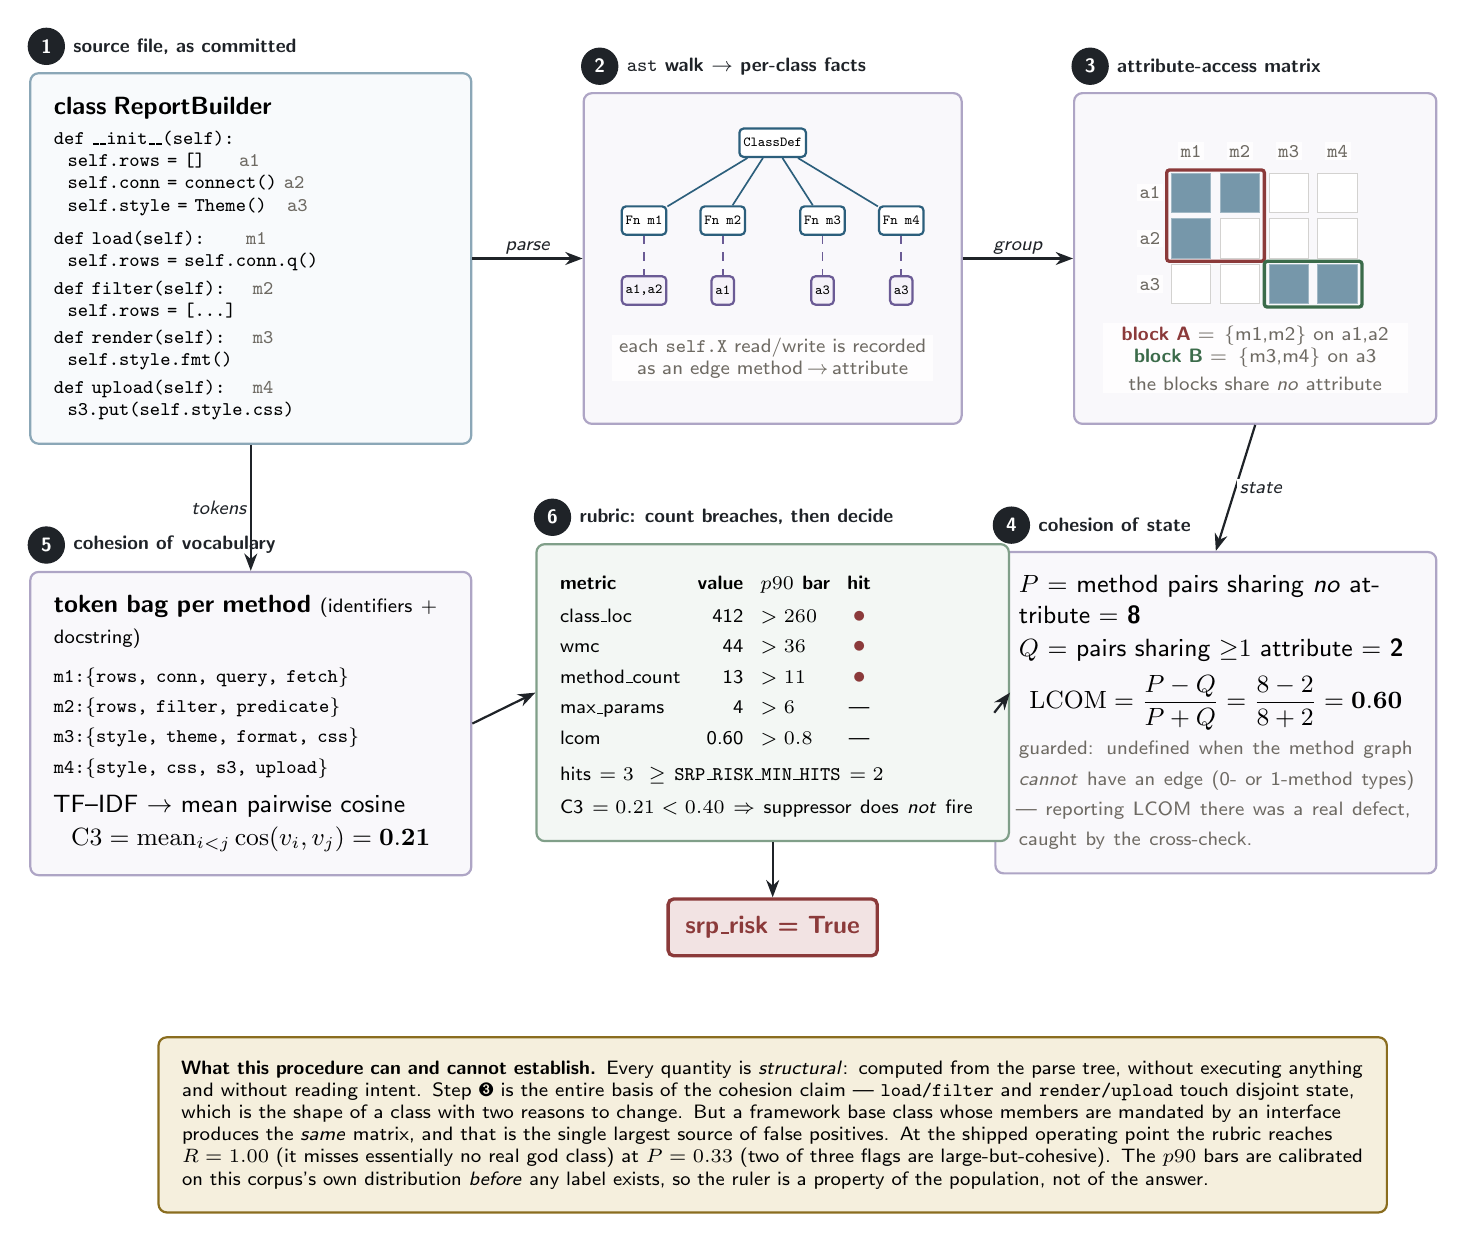
\begin{tikzpicture}[node distance=11mm]

% ===================== 1. SOURCE ===========================================
\node[srcpanel, text width=50mm, font=\ttfamily\scriptsize] (src)
{\textbf{\sffamily\small class ReportBuilder}\\[3pt]
 def \_\_init\_\_(self):\\
 \ \ self.rows\ = []\ \ \ \ \ \textcolor{vbNote}{a1}\\
 \ \ self.conn\ = connect()\ \textcolor{vbNote}{a2}\\
 \ \ self.style = Theme()\ \ \ \textcolor{vbNote}{a3}\\[4pt]
 def load(self):\ \ \ \ \ \ \textcolor{vbNote}{m1}\\
 \ \ self.rows = self.conn.q()\\[2pt]
 def filter(self):\ \ \ \ \textcolor{vbNote}{m2}\\
 \ \ self.rows = [\dots]\\[2pt]
 def render(self):\ \ \ \ \textcolor{vbNote}{m3}\\
 \ \ self.style.fmt()\\[2pt]
 def upload(self):\ \ \ \ \textcolor{vbNote}{m4}\\
 \ \ s3.put(self.style.css)};
\steptitle{src}{1}{source file, as committed}

% ===================== 2. AST ==============================================
\node[calcpanel, right=14mm of src, text width=42mm, minimum height=42mm] (astp) {};
\steptitle{astp}{2}{\texttt{ast} walk $\to$ per-class facts}

\node[astn, anchor=north] at ($(astp.north)+(0,-0.45)$) (ncls) {ClassDef};
\node[astn, below left=6mm and 9mm of ncls] (nm1) {Fn m1};
\node[astn, below left=6mm and -1mm of ncls] (nm2) {Fn m2};
\node[astn, below right=6mm and -1mm of ncls] (nm3) {Fn m3};
\node[astn, below right=6mm and 9mm of ncls] (nm4) {Fn m4};
\foreach \n in {nm1,nm2,nm3,nm4} \draw[semithick,vbStage] (ncls) -- (\n);

\node[astleaf, below=5mm of nm1] (l1) {a1,a2};
\node[astleaf, below=5mm of nm2] (l2) {a1};
\node[astleaf, below=5mm of nm3] (l3) {a3};
\node[astleaf, below=5mm of nm4] (l4) {a3};
\foreach \a/\b in {nm1/l1,nm2/l2,nm3/l3,nm4/l4}
  \draw[semithick,vbStore,dashed] (\a) -- (\b);
\node[lbl, anchor=north, text width=40mm, align=center]
  at ($(astp.south)+(0,1.15)$)
  {each \texttt{self.X} read/write is recorded\\as an edge method\,$\to$\,attribute};

\draw[flow] (src) -- node[wetag,above]{parse} (astp);

% ===================== 3. ACCESS MATRIX ====================================
\node[calcpanel, right=14mm of astp, text width=40mm, minimum height=42mm] (mtxp) {};
\steptitle{mtxp}{3}{attribute-access matrix}

\foreach \m/\j in {m1/0, m2/1, m3/2, m4/3}
  \node[lbl] at ($(mtxp.north west)+(1.5+0.62*\j,-0.75)$) {\texttt{\m}};
\foreach \a/\i in {a1/0, a2/1, a3/2}
  \node[lbl, anchor=east] at ($(mtxp.north west)+(1.15,-1.28-0.58*\i)$) {\texttt{\a}};
\foreach \i/\j/\v in {
  0/0/1, 0/1/1, 0/2/0, 0/3/0,
  1/0/1, 1/1/0, 1/2/0, 1/3/0,
  2/0/0, 2/1/0, 2/2/1, 2/3/1}{
  \ifnum\v=1
    \node[cellon]  at ($(mtxp.north west)+(1.5+0.62*\j,-1.28-0.58*\i)$) {};
  \else
    \node[celloff] at ($(mtxp.north west)+(1.5+0.62*\j,-1.28-0.58*\i)$) {};
  \fi}

% highlight the two disjoint blocks
\draw[vbDrop, very thick, rounded corners=1pt]
  ($(mtxp.north west)+(1.19,-0.99)$) rectangle ($(mtxp.north west)+(2.43,-2.15)$);
\draw[vbGood, very thick, rounded corners=1pt]
  ($(mtxp.north west)+(2.43,-2.15)$) rectangle ($(mtxp.north west)+(3.67,-2.73)$);
\node[lbl, anchor=north, text width=38mm, align=center]
  at ($(mtxp.south)+(0,1.30)$)
  {\textcolor{vbDrop}{\textbf{block A}} $=\{$m1,m2$\}$ on a1,a2\\
   \textcolor{vbGood}{\textbf{block B}} $=\{$m3,m4$\}$ on a3\\[2pt]
   the blocks share \emph{no} attribute};

\draw[flow] (astp) -- node[wetag,above]{group} (mtxp);

% ===================== 4. LCOM =============================================
\node[calcpanel, below=16mm of mtxp.south east, anchor=north east, text width=50mm] (lcom)
{$P$ = method pairs sharing \emph{no} attribute = \textbf{8}\\[1pt]
 $Q$ = pairs sharing ${\geq}1$ attribute = \textbf{2}\\[4pt]
 \mbox{}\hfill$\mathrm{LCOM}=\dfrac{P-Q}{P+Q}=\dfrac{8-2}{8+2}=\mathbf{0.60}$\hfill\mbox{}\\[3pt]
 \textcolor{vbNote}{\scriptsize guarded: undefined when the method graph
 \emph{cannot} have an edge (0- or 1-method types) --- reporting LCOM there was a
 real defect, caught by the cross-check.}};
\steptitle{lcom}{4}{cohesion of \emph{state}}

% ===================== 5. C3 ===============================================
\node[calcpanel, below=16mm of src.south west, anchor=north west, text width=50mm] (c3)
{\textbf{token bag per method} {\scriptsize(identifiers + docstring)}\\[3pt]
 {\ttfamily\scriptsize m1:\{rows, conn, query, fetch\}}\\
 {\ttfamily\scriptsize m2:\{rows, filter, predicate\}}\\
 {\ttfamily\scriptsize m3:\{style, theme, format, css\}}\\
 {\ttfamily\scriptsize m4:\{style, css, s3, upload\}}\\[3pt]
 TF--IDF $\to$ mean pairwise cosine\\[1pt]
 \mbox{}\hfill$\mathrm{C3}=\operatorname{mean}_{i<j}\cos(v_i,v_j)=\mathbf{0.21}$\hfill\mbox{}};
\steptitle{c3}{5}{cohesion of \emph{vocabulary}}




% ===================== 6. RUBRIC ===========================================
\node[outpanel, below=15mm of astp.south, anchor=north, text width=54mm] (rub)
{\begin{tabular}{@{}l@{\ \ }r@{\ \ }l@{\ \ }c@{}}
 \textbf{\scriptsize metric} & \textbf{\scriptsize value} & \textbf{\scriptsize $p90$ bar} & \textbf{\scriptsize hit}\\[1pt]
 {\scriptsize class\_loc}    & {\scriptsize 412}  & {\scriptsize $>260$} & \textcolor{vbDrop}{$\bullet$}\\
 {\scriptsize wmc}           & {\scriptsize 44}   & {\scriptsize $>36$}  & \textcolor{vbDrop}{$\bullet$}\\
 {\scriptsize method\_count} & {\scriptsize 13}   & {\scriptsize $>11$}  & \textcolor{vbDrop}{$\bullet$}\\
 {\scriptsize max\_params}   & {\scriptsize 4}    & {\scriptsize $>6$}   & {\scriptsize ---}\\
 {\scriptsize lcom}          & {\scriptsize 0.60} & {\scriptsize $>0.8$} & {\scriptsize ---}\\
 \end{tabular}\\[4pt]
 {\scriptsize hits $=3\ \geq$ \texttt{SRP\_RISK\_MIN\_HITS} $=2$}\\[1pt]
 {\scriptsize C3 $=0.21<0.40$ $\Rightarrow$ suppressor does \emph{not} fire}};
\steptitle{rub}{6}{rubric: count breaches, then decide}


\draw[flow] (mtxp.south) -- node[wetag,right]{state} (lcom.north);
\draw[flow] (src.south) -- node[wetag,left]{tokens} (c3.north);
\draw[flow] (c3.east) -- (rub.west);
\draw[flow] (lcom.west) -- (rub.east);

\node[verdict, below=7mm of rub] (verd) {srp\_risk = True};
\draw[flow] (rub) -- (verd);

% ===================== caveat ==============================================
\node[panel, draw=vbWarn, fill=vbWarnBg, font=\sffamily\scriptsize,
      below=10mm of verd.south, anchor=north, text width=150mm] (warn)
{\textbf{What this procedure can and cannot establish.} Every quantity is \emph{structural}:
 computed from the parse tree, without executing anything and without reading intent. Step
 \ding{204} is the entire basis of the cohesion claim --- \texttt{load/filter} and
 \texttt{render/upload} touch disjoint state, which is the shape of a class with two reasons to
 change. But a framework base class whose members are mandated by an interface produces the
 \emph{same} matrix, and that is the single largest source of false positives. At the shipped
 operating point the rubric reaches $R=1.00$ (it misses essentially no real god class) at
 $P=0.33$ (two of three flags are large-but-cohesive). The $p90$ bars are calibrated on this
 corpus's own distribution \emph{before} any label exists, so the ruler is a property of the
 population, not of the answer.};

\end{tikzpicture}}
\caption{\textbf{SRP detector, worked end to end on a single class.} Boxes shaded blue are
inputs, purple are intermediate computations, green is the decision.}
\end{figure}

\clearpage

% =====================================================================
\section*{7. DIP detector, worked end to end}
% =====================================================================

\begin{figure}[h]
\centering
\fitpic{%
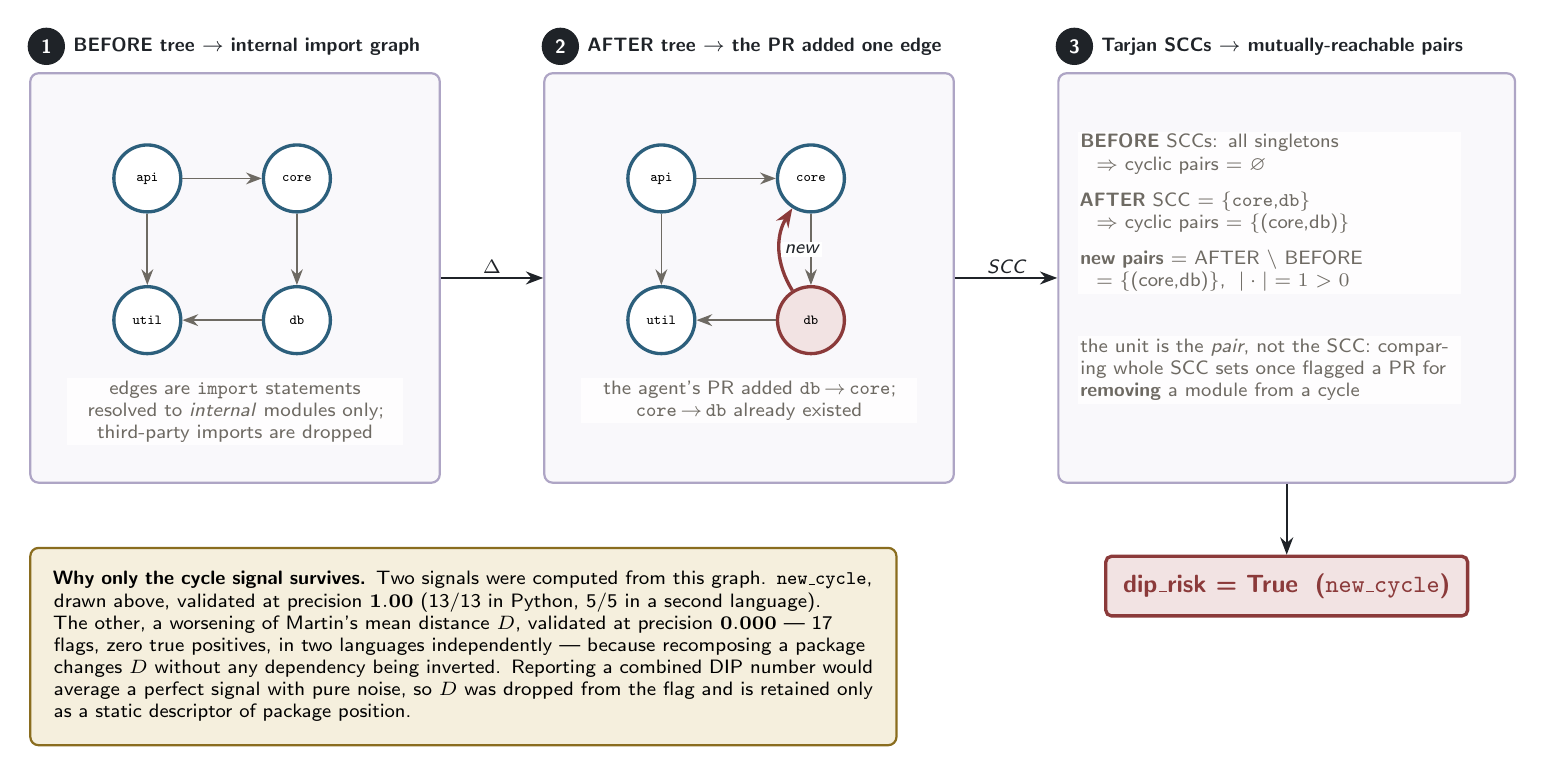
\begin{tikzpicture}

% ---------- BEFORE graph ----------
\node[calcpanel, text width=46mm, minimum height=52mm] (bef) {};
\steptitle{bef}{1}{BEFORE tree $\to$ internal import graph}

\node[mod] at ($(bef.north west)+(1.5,-1.35)$) (b_api)  {api};
\node[mod] at ($(bef.north west)+(3.4,-1.35)$) (b_core) {core};
\node[mod] at ($(bef.north west)+(1.5,-3.15)$) (b_util) {util};
\node[mod] at ($(bef.north west)+(3.4,-3.15)$) (b_db)   {db};
\draw[imp] (b_api)  -- (b_core);
\draw[imp] (b_core) -- (b_db);
\draw[imp] (b_api)  -- (b_util);
\draw[imp] (b_db)   -- (b_util);
\node[lbl, anchor=north, text width=42mm, align=center] at ($(bef.south)+(0,1.35)$)
  {edges are \texttt{import} statements resolved to \emph{internal} modules only;\\
   third-party imports are dropped};

% ---------- AFTER graph ----------
\node[calcpanel, right=13mm of bef, text width=46mm, minimum height=52mm] (aft) {};
\steptitle{aft}{2}{AFTER tree $\to$ the PR added one edge}

\node[mod]    at ($(aft.north west)+(1.5,-1.35)$) (a_api)  {api};
\node[mod]    at ($(aft.north west)+(3.4,-1.35)$) (a_core) {core};
\node[mod]    at ($(aft.north west)+(1.5,-3.15)$) (a_util) {util};
\node[modnew] at ($(aft.north west)+(3.4,-3.15)$) (a_db)   {db};
\draw[imp] (a_api)  -- (a_core);
\draw[imp] (a_core) -- (a_db);
\draw[imp] (a_api)  -- (a_util);
\draw[imp] (a_db)   -- (a_util);
\draw[impnew] (a_db) to[bend left=32] node[wetag,right,pos=0.5]{new} (a_core);
\node[lbl, anchor=north, text width=42mm, align=center] at ($(aft.south)+(0,1.35)$)
  {the agent's PR added \texttt{db}\,$\to$\,\texttt{core};\\
   \texttt{core}\,$\to$\,\texttt{db} already existed};

\draw[flow] (bef) -- node[wetag,above]{$\Delta$} (aft);

% ---------- Tarjan ----------
\node[calcpanel, right=13mm of aft, text width=52mm, minimum height=52mm] (tar) {};
\steptitle{tar}{3}{Tarjan SCCs $\to$ mutually-reachable pairs}

\node[lbl, anchor=north west, text width=48mm, align=left] at ($(tar.north west)+(0.25,-0.75)$)
 {\textbf{BEFORE} SCCs: all singletons\\
  \hspace*{2mm}$\Rightarrow$ cyclic pairs $=\varnothing$\\[5pt]
  \textbf{AFTER} SCC $=\{$\texttt{core},\texttt{db}$\}$\\
  \hspace*{2mm}$\Rightarrow$ cyclic pairs $=\{$(core,db)$\}$\\[5pt]
  \textbf{new pairs} $=$ AFTER $\setminus$ BEFORE\\
  \hspace*{2mm}$=\{$(core,db)$\}$, \;$|\cdot|=1>0$};

\node[lbl, anchor=north west, text width=48mm, align=left, text=vbNote]
  at ($(tar.north west)+(0.25,-3.35)$)
 {the unit is the \emph{pair}, not the SCC: comparing whole SCC sets once flagged a PR for
  \textbf{removing} a module from a cycle};

\draw[flow] (aft) -- node[wetag,above]{SCC} (tar);

\node[verdict, below=9mm of tar] (v1) {dip\_risk = True \;(\texttt{new\_cycle})};
\draw[flow] (tar) -- (v1);

% ---------- caveat ----------
\node[panel, draw=vbWarn, fill=vbWarnBg, font=\sffamily\scriptsize,
      below=8mm of bef.south west, anchor=north west, text width=104mm] (w1)
{\textbf{Why only the cycle signal survives.} Two signals were computed from this graph.
 \texttt{new\_cycle}, drawn above, validated at precision $\mathbf{1.00}$ (13/13 in Python,
 5/5 in a second language). The other, a worsening of Martin's mean distance $D$, validated at
 precision $\mathbf{0.000}$ --- 17 flags, zero true positives, in two languages independently ---
 because recomposing a package changes $D$ without any dependency being inverted. Reporting a
 combined DIP number would average a perfect signal with pure noise, so $D$ was dropped from
 the flag and is retained only as a static descriptor of package position.};

\end{tikzpicture}}
\caption{\textbf{DIP detector: the same graph before and after, and the pair that appeared.}
Circles are internal modules, arrows are resolved imports. Only edges between modules of the
repository itself are kept, so a dependency on an external library is invisible by
construction.}
\end{figure}

\clearpage

% =====================================================================
\section*{8. OCP detector, worked end to end}
% =====================================================================

\begin{figure}[h]
\centering
\fitpic{%
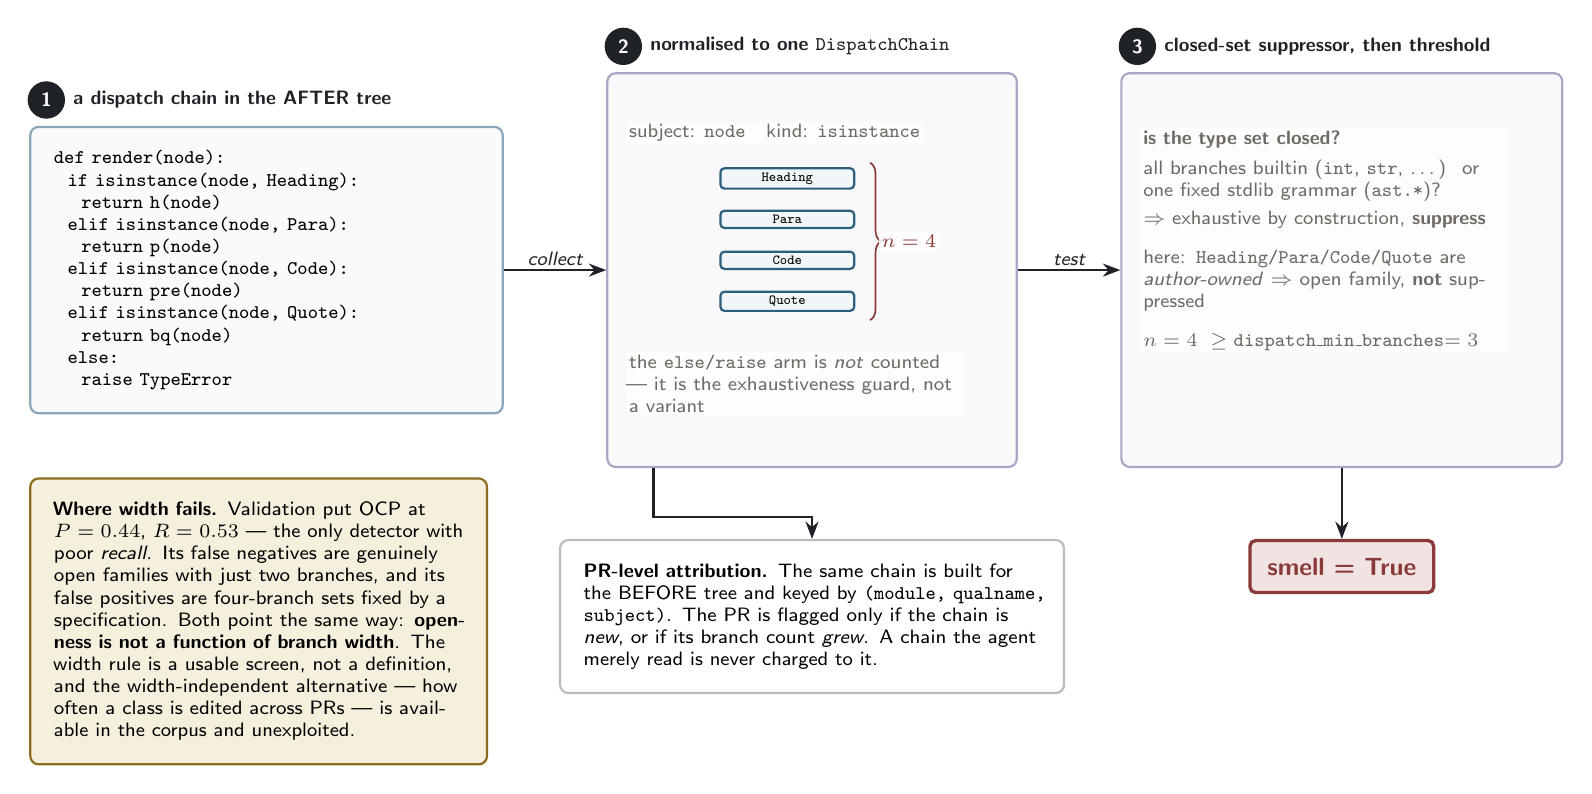
\begin{tikzpicture}

% ---------- source ----------
\node[srcpanel, text width=54mm, font=\ttfamily\scriptsize] (osrc)
{def render(node):\\
 \ \ \textbf{if} isinstance(node, Heading):\\
 \ \ \ \ return h(node)\\
 \ \ \textbf{elif} isinstance(node, Para):\\
 \ \ \ \ return p(node)\\
 \ \ \textbf{elif} isinstance(node, Code):\\
 \ \ \ \ return pre(node)\\
 \ \ \textbf{elif} isinstance(node, Quote):\\
 \ \ \ \ return bq(node)\\
 \ \ \textbf{else}:\\
 \ \ \ \ raise TypeError};
\steptitle{osrc}{1}{a dispatch chain in the AFTER tree}

% ---------- chain object ----------
\node[calcpanel, right=13mm of osrc, text width=46mm, minimum height=50mm] (ochain) {};
\steptitle{ochain}{2}{normalised to one \texttt{DispatchChain}}

\node[lbl, anchor=north west] at ($(ochain.north west)+(0.25,-0.62)$)
  {subject: \texttt{node}\quad kind: \texttt{isinstance}};
\foreach \n/\i in {Heading/0, Para/1, Code/2, Quote/3}
  \node[brc] at ($(ochain.north west)+(2.3,-1.35-0.52*\i)$) {\n};
\draw[decorate, decoration={brace, amplitude=4pt}, semithick, vbDrop]
  ($(ochain.north west)+(3.35,-1.15)$) -- ($(ochain.north west)+(3.35,-3.15)$)
  node[midway, right=3pt, lbl, text=vbDrop] {$n=4$};
\node[lbl, anchor=north west, text width=42mm] at ($(ochain.north west)+(0.25,-3.55)$)
  {the \texttt{else/raise} arm is \emph{not} counted --- it is the exhaustiveness guard,
   not a variant};

\draw[flow] (osrc) -- node[wetag,above]{collect} (ochain);

% ---------- closed-set test + decision ----------
\node[calcpanel, right=13mm of ochain, text width=50mm, minimum height=50mm] (otest) {};
\steptitle{otest}{3}{closed-set suppressor, then threshold}

\node[lbl, anchor=north west, text width=46mm, align=left] at ($(otest.north west)+(0.25,-0.70)$)
 {\textbf{is the type set closed?}\\[3pt]
  all branches builtin (\texttt{int}, \texttt{str}, \dots) \;or\; one fixed stdlib grammar
  (\texttt{ast.*})?\\[2pt]
  $\Rightarrow$ exhaustive by construction, \textbf{suppress}\\[6pt]
  here: \texttt{Heading/Para/Code/Quote} are \emph{author-owned} $\Rightarrow$ open family,
  \textbf{not} suppressed\\[6pt]
  $n=4 \;\geq\;$\texttt{dispatch\_min\_branches}$=3$};

\draw[flow] (ochain) -- node[wetag,above]{test} (otest);
\node[verdict, below=9mm of otest] (v2) {smell = True};
\draw[flow] (otest) -- (v2);

% ---------- delta note ----------
\node[panel, draw=vbNote!45, fill=white, font=\sffamily\scriptsize,
      below=9mm of ochain.south, anchor=north, text width=58mm] (dnote)
{\textbf{PR-level attribution.} The same chain is built for the BEFORE tree and keyed by
 \texttt{(module, qualname, subject)}. The PR is flagged only if the chain is
 \emph{new}, or if its branch count \emph{grew}. A chain the agent merely read is never
 charged to it.};
\draw[flow] (ochain.south west) ++(0.6,0) -- ++(0,-0.62) -| (dnote.north);

% ---------- caveat ----------
\node[panel, draw=vbWarn, fill=vbWarnBg, font=\sffamily\scriptsize,
      below=8mm of osrc.south west, anchor=north west, text width=52mm] (w2)
{\textbf{Where width fails.} Validation put OCP at $P=0.44$, $R=0.53$ --- the only detector
 with poor \emph{recall}. Its false negatives are genuinely open families with just two
 branches, and its false positives are four-branch sets fixed by a specification. Both point
 the same way: \textbf{openness is not a function of branch width}. The width rule is a
 usable screen, not a definition, and the width-independent alternative --- how often a class
 is edited across PRs --- is available in the corpus and unexploited.};

\end{tikzpicture}}
\caption{\textbf{OCP detector: from an \texttt{isinstance} ladder to a flag.} The chain is the
unit of analysis; the branch count is the measurement; the closed-set test is the one
deterministic correction that survived validation.}
\end{figure}

\clearpage

% =====================================================================
\section*{9. LSP detector, worked end to end}
% =====================================================================

\begin{figure}[h]
\centering
\fitpic{%
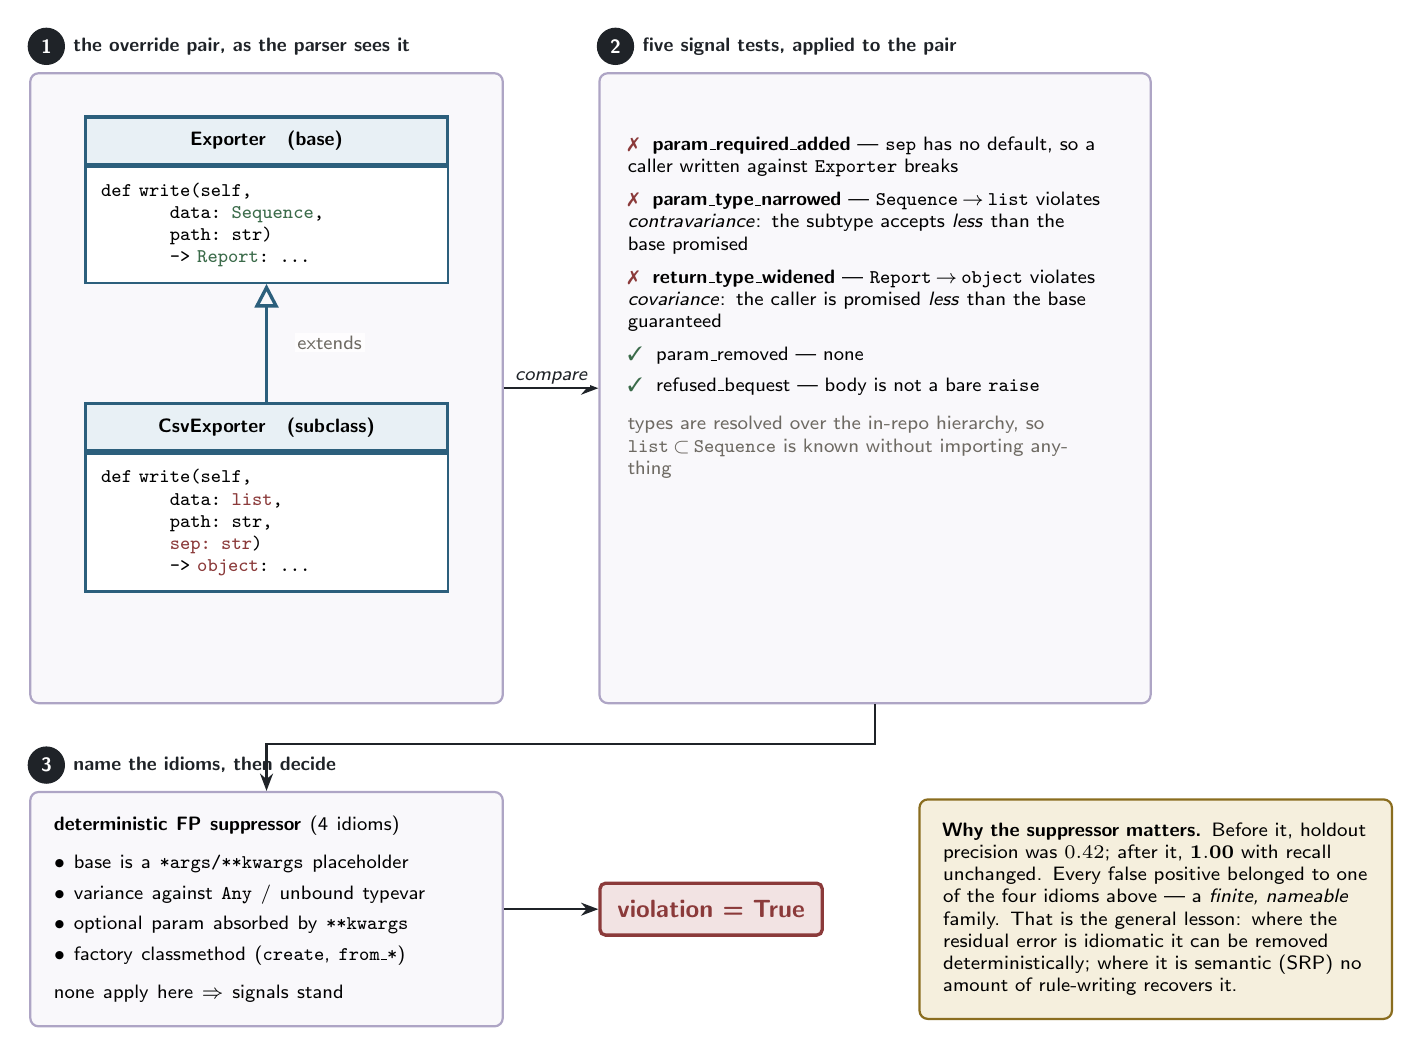
\begin{tikzpicture}

% ---------- the hierarchy ----------
\node[calcpanel, text width=54mm, minimum height=80mm] (hier) {};
\steptitle{hier}{1}{the override pair, as the parser sees it}

\node[clshdr, anchor=north] at ($(hier.north)+(0,-0.55)$) (bh) {Exporter \ \ {\scriptsize(base)}};
\node[clsbody, anchor=north] at (bh.south) (bb)
 {def write(self,\\
  \ \ \ \ \ \ \ \ \ \ data: \textcolor{vbGood}{\textbf{Sequence}},\\
  \ \ \ \ \ \ \ \ \ \ path: str)\\
  \ \ \ \ \ \ \ \ \ \ -> \textcolor{vbGood}{\textbf{Report}}: ...};

\node[clshdr, anchor=north] at ($(bb.south)+(0,-1.5)$) (sh) {CsvExporter \ \ {\scriptsize(subclass)}};
\node[clsbody, anchor=north] at (sh.south) (sb)
 {def write(self,\\
  \ \ \ \ \ \ \ \ \ \ data: \textcolor{vbDrop}{\textbf{list}},\\
  \ \ \ \ \ \ \ \ \ \ path: str,\\
  \ \ \ \ \ \ \ \ \ \ \textcolor{vbDrop}{\textbf{sep: str}})\\
  \ \ \ \ \ \ \ \ \ \ -> \textcolor{vbDrop}{\textbf{object}}: ...};

\draw[inherit] (sh.north) -- ($(bb.south)+(0,0)$);
\node[lbl, anchor=west] at ($(sh.north)!0.5!(bb.south)+(0.35,0)$) {extends};

% ---------- signal tests ----------
\node[calcpanel, right=12mm of hier, text width=64mm, minimum height=80mm] (sig) {};
\steptitle{sig}{2}{five signal tests, applied to the pair}

\node[anchor=north west, text width=60mm, font=\sffamily\scriptsize, align=left]
  at ($(sig.north west)+(0.25,-0.70)$)
 {\textcolor{vbDrop}{\ding{55}}\ \ \textbf{param\_required\_added} --- \texttt{sep} has no
   default, so a caller written against \texttt{Exporter} breaks\\[4pt]
  \textcolor{vbDrop}{\ding{55}}\ \ \textbf{param\_type\_narrowed} ---
   \texttt{Sequence}$\,\to\,$\texttt{list} violates \emph{contravariance}: the subtype accepts
   \emph{less} than the base promised\\[4pt]
  \textcolor{vbDrop}{\ding{55}}\ \ \textbf{return\_type\_widened} ---
   \texttt{Report}$\,\to\,$\texttt{object} violates \emph{covariance}: the caller is promised
   \emph{less} than the base guaranteed\\[4pt]
  \textcolor{vbGood}{\ding{51}}\ \ param\_removed --- none\\[3pt]
  \textcolor{vbGood}{\ding{51}}\ \ refused\_bequest --- body is not a bare \texttt{raise}\\[6pt]
  \textcolor{vbNote}{types are resolved over the in-repo hierarchy, so
   \texttt{list}$\,\subset\,$\texttt{Sequence} is known without importing anything}};

\draw[flow] (hier) -- node[wetag,above]{compare} (sig);

% ---------- suppressor + verdict ----------
\node[calcpanel, below=11mm of hier.south west, anchor=north west,
      text width=54mm] (sup)
{\textbf{\scriptsize deterministic FP suppressor} {\scriptsize(4 idioms)}\\[3pt]
 {\scriptsize $\bullet$ base is a \texttt{*args/**kwargs} placeholder}\\
 {\scriptsize $\bullet$ variance against \texttt{Any} / unbound typevar}\\
 {\scriptsize $\bullet$ optional param absorbed by \texttt{**kwargs}}\\
 {\scriptsize $\bullet$ factory classmethod (\texttt{create}, \texttt{from\_*})}\\[3pt]
 {\scriptsize none apply here $\Rightarrow$ signals stand}};
\steptitle{sup}{3}{name the idioms, then decide}
\draw[flow] (sig.south) -- ++(0,-0.5) -| (sup.north);

\node[verdict, right=12mm of sup] (v) {violation = True};
\draw[flow] (sup) -- (v);

\node[panel, draw=vbWarn, fill=vbWarnBg, font=\sffamily\scriptsize,
      right=12mm of v, text width=54mm] (w)
{\textbf{Why the suppressor matters.} Before it, holdout precision was $0.42$; after it,
 $\mathbf{1.00}$ with recall unchanged. Every false positive belonged to one of the four
 idioms above --- a \emph{finite, nameable} family. That is the general lesson: where the
 residual error is idiomatic it can be removed deterministically; where it is semantic
 (SRP) no amount of rule-writing recovers it.};

\end{tikzpicture}}
\caption{\textbf{LSP detector: one override pair, five tests.} The rule replicates what a type
checker would report, on the AST, because 147 repositories cannot be made importable. Which
signals are even \emph{expressible} is language-dependent: \texttt{javac} makes three of these
impossible in code that compiles, so the Java signal set keeps only what a compiler cannot check.}
\end{figure}

\clearpage

% =====================================================================
\section*{10. ISP detector, worked end to end}
% =====================================================================

\begin{figure}[h]
\centering
\fitpic{%
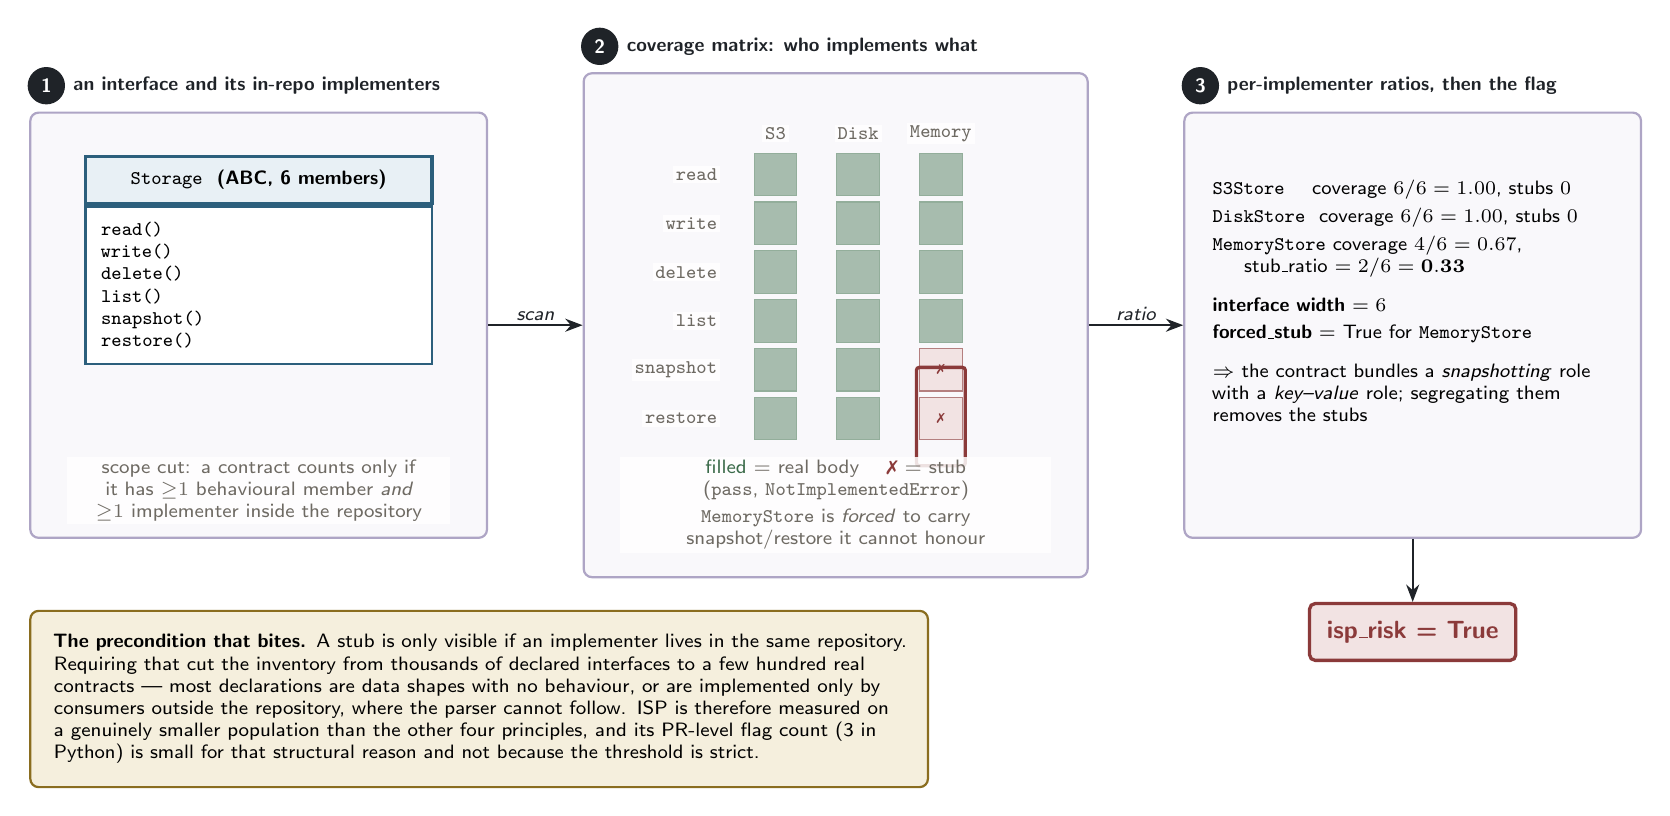
\begin{tikzpicture}

% ---------- the contract ----------
\node[calcpanel, text width=52mm, minimum height=54mm] (ifc) {};
\steptitle{ifc}{1}{an interface and its in-repo implementers}

\node[clshdr, anchor=north, minimum width=44mm] at ($(ifc.north)+(0,-0.55)$) (ih)
  {\texttt{Storage} \ {\scriptsize(ABC, 6 members)}};
\node[clsbody, anchor=north, minimum width=44mm, text width=40mm] at (ih.south) (ib)
 {read()\\ write()\\ delete()\\ list()\\ snapshot()\\ restore()};

\node[lbl, anchor=north, text width=48mm, align=center] at ($(ifc.south)+(0,1.05)$)
 {scope cut: a contract counts only if it has ${\geq}1$ behavioural member \emph{and}
  ${\geq}1$ implementer inside the repository};

% ---------- coverage matrix ----------
\node[calcpanel, right=12mm of ifc, text width=58mm, minimum height=64mm] (cov) {};
\steptitle{cov}{2}{coverage matrix: who implements what}

\foreach \m/\i in {read/0, write/1, delete/2, list/3, snapshot/4, restore/5}
  \node[lbl, anchor=east] at ($(cov.north west)+(1.75,-1.30-0.62*\i)$) {\texttt{\m}};
\foreach \c/\j in {S3/0, Disk/1, Memory/2}
  \node[lbl] at ($(cov.north west)+(2.45+1.05*\j,-0.78)$) {\texttt{\c}};

% S3: all implemented; Disk: all; Memory: 4 impl + 2 stubs
\foreach \i in {0,1,2,3,4,5}{
  \node[impl] at ($(cov.north west)+(2.45,-1.30-0.62*\i)$) {};
  \node[impl] at ($(cov.north west)+(3.50,-1.30-0.62*\i)$) {};}
\foreach \i in {0,1,2,3}
  \node[impl] at ($(cov.north west)+(4.55,-1.30-0.62*\i)$) {};
\foreach \i in {4,5}
  \node[stub] at ($(cov.north west)+(4.55,-1.30-0.62*\i)$) {\ding{55}};

\draw[vbDrop, very thick, rounded corners=1pt]
  ($(cov.north west)+(4.24,-3.75)$) rectangle ($(cov.north west)+(4.86,-5.00)$);

\node[lbl, anchor=north, text width=54mm, align=center] at ($(cov.south)+(0,1.55)$)
 {\textcolor{vbGood}{filled} $=$ real body \quad
  \textcolor{vbDrop}{\ding{55}} $=$ stub (\texttt{pass}, \texttt{NotImplementedError})\\[2pt]
  \texttt{MemoryStore} is \emph{forced} to carry snapshot/restore it cannot honour};

\draw[flow] (ifc) -- node[wetag,above]{scan} (cov);

% ---------- ratios + verdict ----------
\node[calcpanel, right=12mm of cov, text width=52mm, minimum height=54mm] (rat) {};
\steptitle{rat}{3}{per-implementer ratios, then the flag}

\node[anchor=north west, text width=48mm, font=\sffamily\scriptsize, align=left]
  at ($(rat.north west)+(0.25,-0.75)$)
 {\texttt{S3Store}\ \ \ \ coverage $6/6=1.00$, stubs $0$\\[2pt]
  \texttt{DiskStore}\ \ coverage $6/6=1.00$, stubs $0$\\[2pt]
  \texttt{MemoryStore} coverage $4/6=0.67$,\\
  \hspace*{4mm}stub\_ratio $=2/6=\mathbf{0.33}$\\[6pt]
  \textbf{interface width} $=6$\\[2pt]
  \textbf{forced\_stub} $=$ True for \texttt{MemoryStore}\\[6pt]
  $\Rightarrow$ the contract bundles a \emph{snapshotting} role with a
  \emph{key--value} role; segregating them removes the stubs};

\draw[flow] (cov) -- node[wetag,above]{ratio} (rat);
\node[verdict, below=8mm of rat] (v2) {isp\_risk = True};
\draw[flow] (rat) -- (v2);

\node[panel, draw=vbWarn, fill=vbWarnBg, font=\sffamily\scriptsize,
      below=9mm of ifc.south west, anchor=north west, text width=108mm] (w2)
{\textbf{The precondition that bites.} A stub is only visible if an implementer lives in the
 same repository. Requiring that cut the inventory from thousands of declared interfaces to a
 few hundred real contracts --- most declarations are data shapes with no behaviour, or are
 implemented only by consumers outside the repository, where the parser cannot follow. ISP is
 therefore measured on a genuinely smaller population than the other four principles, and its
 PR-level flag count (3 in Python) is small for that structural reason and not because the
 threshold is strict.};

\end{tikzpicture}}
\caption{\textbf{ISP detector: interface width against what implementers actually use.} The
matrix is the measurement; a column with stubbed cells is a client paying for members it does
not need.}
\end{figure}

\clearpage

% =====================================================================
\section*{11. The proxies: what is asserted vs.\ what is computed}
% =====================================================================

\begin{figure}[h]
\centering
\fitpic{%
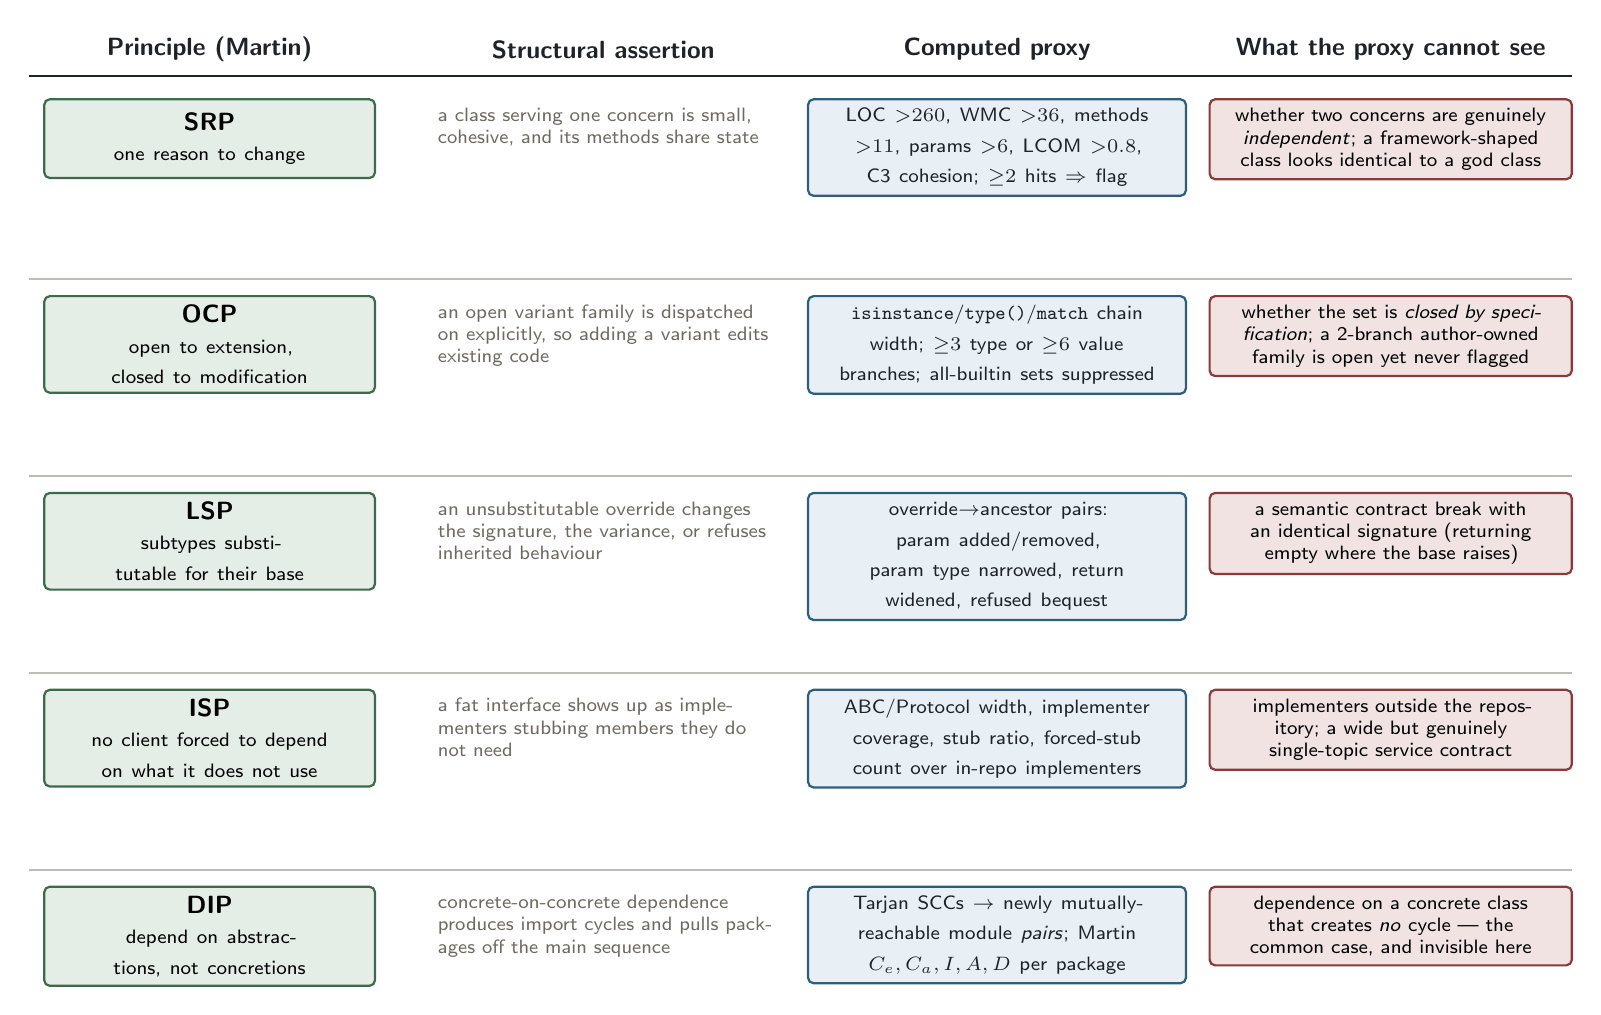
\begin{tikzpicture}

% ---- column headers ----
\node[font=\sffamily\bfseries\small, text=vbInk] at (0,0)    {Principle (Martin)};
\node[font=\sffamily\bfseries\small, text=vbInk] at (5.0,0)  {Structural assertion};
\node[font=\sffamily\bfseries\small, text=vbInk] at (10.0,0) {Computed proxy};
\node[font=\sffamily\bfseries\small, text=vbInk] at (15.0,0) {What the proxy cannot see};
\draw[semithick, vbInk] (-2.3,-0.34) -- (17.3,-0.34);

% ---- SRP ----
\node[keep, text width=36mm, anchor=north] at (0,-0.62)
  {\textbf{SRP}\\{\scriptsize one reason to change}};
\node[note, text width=42mm, anchor=north] at (5.0,-0.62)
  {a class serving one concern is small, cohesive, and its methods share state};
\node[stage, text width=42mm, anchor=north] at (10.0,-0.62)
  {{\scriptsize LOC ${>}260$, WMC ${>}36$, methods ${>}11$, params ${>}6$, LCOM ${>}0.8$, C3 cohesion; ${\geq}2$ hits $\Rightarrow$ flag}};
\node[drop, text width=42mm, anchor=north] at (15.0,-0.62)
  {whether two concerns are genuinely \emph{independent}; a framework-shaped class looks identical to a god class};

% ---- OCP ----
\node[keep, text width=36mm, anchor=north] at (0,-3.12)
  {\textbf{OCP}\\{\scriptsize open to extension, closed to modification}};
\node[note, text width=42mm, anchor=north] at (5.0,-3.12)
  {an open variant family is dispatched on explicitly, so adding a variant edits existing code};
\node[stage, text width=42mm, anchor=north] at (10.0,-3.12)
  {{\scriptsize \texttt{isinstance}/\texttt{type()}/\texttt{match} chain width; ${\geq}3$ type or ${\geq}6$ value branches; all-builtin sets suppressed}};
\node[drop, text width=42mm, anchor=north] at (15.0,-3.12)
  {whether the set is \emph{closed by specification}; a 2-branch author-owned family is open yet never flagged};

% ---- LSP ----
\node[keep, text width=36mm, anchor=north] at (0,-5.62)
  {\textbf{LSP}\\{\scriptsize subtypes substitutable for their base}};
\node[note, text width=42mm, anchor=north] at (5.0,-5.62)
  {an unsubstitutable override changes the signature, the variance, or refuses inherited behaviour};
\node[stage, text width=42mm, anchor=north] at (10.0,-5.62)
  {{\scriptsize override$\to$ancestor pairs: param added/removed, param type narrowed, return widened, refused bequest}};
\node[drop, text width=42mm, anchor=north] at (15.0,-5.62)
  {a semantic contract break with an identical signature (returning empty where the base raises)};

% ---- ISP ----
\node[keep, text width=36mm, anchor=north] at (0,-8.12)
  {\textbf{ISP}\\{\scriptsize no client forced to depend on what it does not use}};
\node[note, text width=42mm, anchor=north] at (5.0,-8.12)
  {a fat interface shows up as implementers stubbing members they do not need};
\node[stage, text width=42mm, anchor=north] at (10.0,-8.12)
  {{\scriptsize ABC/Protocol width, implementer coverage, stub ratio, forced-stub count over in-repo implementers}};
\node[drop, text width=42mm, anchor=north] at (15.0,-8.12)
  {implementers outside the repository; a wide but genuinely single-topic service contract};

% ---- DIP ----
\node[keep, text width=36mm, anchor=north] at (0,-10.62)
  {\textbf{DIP}\\{\scriptsize depend on abstractions, not concretions}};
\node[note, text width=42mm, anchor=north] at (5.0,-10.62)
  {concrete-on-concrete dependence produces import cycles and pulls packages off the main sequence};
\node[stage, text width=42mm, anchor=north] at (10.0,-10.62)
  {{\scriptsize Tarjan SCCs $\to$ newly mutually-reachable module \emph{pairs}; Martin $C_e,C_a,I,A,D$ per package}};
\node[drop, text width=42mm, anchor=north] at (15.0,-10.62)
  {dependence on a concrete class that creates \emph{no} cycle --- the common case, and invisible here};

\draw[semithick, vbNote!45] (-2.3,-2.92)  -- (17.3,-2.92);
\draw[semithick, vbNote!45] (-2.3,-5.42)  -- (17.3,-5.42);
\draw[semithick, vbNote!45] (-2.3,-7.92)  -- (17.3,-7.92);
\draw[semithick, vbNote!45] (-2.3,-10.42) -- (17.3,-10.42);

\end{tikzpicture}}
\caption{\textbf{Each principle and the structural proxy that stands in for it.} SOLID is
stated in terms of \emph{reasons to change} and \emph{substitutability} --- semantic properties
no parser can read directly. Every entry in column three is therefore a structural stand-in for
the claim in column two, and column four names exactly what that substitution gives up. The
proxies are not the principles; the next figure measures how far apart they actually are.}
\end{figure}

\clearpage

% =====================================================================
\section*{12. How far is each proxy from its principle?}
% =====================================================================

\begin{figure}[h]
\centering
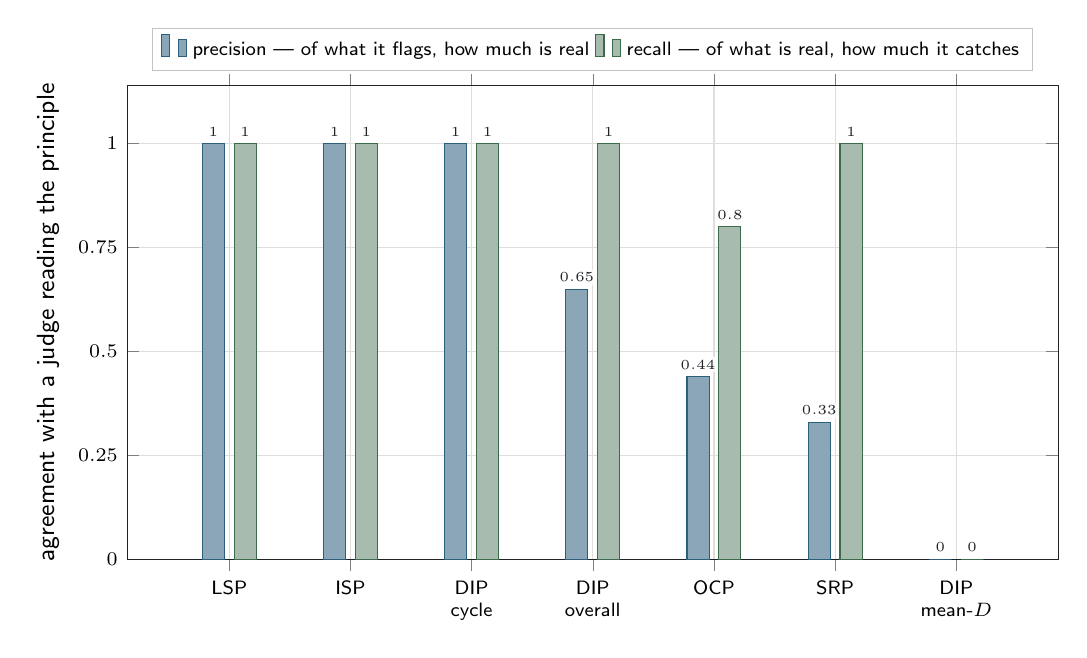
\begin{tikzpicture}
\begin{axis}[
  width=13.4cm, height=7.6cm,
  ybar=3.5pt,
  bar width=8pt,
  enlarge x limits=0.14,
  ymin=0, ymax=1.14,
  ytick={0,0.25,0.5,0.75,1.0},
  ylabel={agreement with a judge reading the principle},
  symbolic x coords={LSP,ISP,DIPcycle,DIPall,OCP,SRP,DIPmeanD},
  xticklabels={LSP, ISP, {DIP\\cycle}, {DIP\\overall}, OCP, SRP, {DIP\\mean-$D$}},
  xtick=data,
  x tick label style={font=\sffamily\scriptsize, align=center, anchor=north},
  tick label style={font=\sffamily\scriptsize},
  label style={font=\sffamily\small},
  legend style={font=\sffamily\scriptsize, at={(0.5,1.03)}, anchor=south,
                legend columns=2, draw=vbNote!40},
  grid=major, grid style={draw=vbNote!22},
  axis line style={vbInk},
  nodes near coords,
  every node near coord/.append style={font=\sffamily\tiny, text=vbInk,
      anchor=south, yshift=1.5pt, inner sep=1pt,
      fill=white, fill opacity=0.85, text opacity=1},
]
\addplot[draw=vbStage, fill=vbStage!55] coordinates
  {(LSP,1.00) (ISP,1.00) (DIPcycle,1.00) (DIPall,0.65) (OCP,0.44) (SRP,0.33) (DIPmeanD,0.00)};
\addplot[draw=vbGood, fill=vbGood!45] coordinates
  {(LSP,1.00) (ISP,1.00) (DIPcycle,1.00) (DIPall,1.00) (OCP,0.80) (SRP,1.00) (DIPmeanD,0.00)};
\legend{precision --- of what it flags{,} how much is real,
        recall --- of what is real{,} how much it catches}
\end{axis}
\end{tikzpicture}
\caption{\textbf{Proxy fidelity is a property of the principle, not of the effort spent.}
Python holdout figures from the completed validation round. The ordering is itself the result.
Where a principle's definition is already \emph{structural}, the proxy very nearly is the
principle: LSP, ISP and DIP's cycle signal all reach precision $1.00$. Where the definition is
\emph{semantic}, structure bounds recall but cannot recover precision --- SRP catches
essentially every real god class ($R{=}1.00$) while two of every three flags are
large-but-cohesive classes. OCP sits between, and its errors explain why: the false positives
are specification-closed sets and the false negatives are narrow author-owned ones, which
together say that openness is not a function of branch width. The two DIP bars are the sharpest
evidence available --- \emph{one principle, two proxies, precision $1.00$ and $0.00$}. Proxy
fidelity must therefore be measured per signal, never assumed per principle.}
\end{figure}

\clearpage

% =====================================================================
\section*{13. Martin's abstractness--instability plane}
% =====================================================================

\begin{figure}[h]
\centering
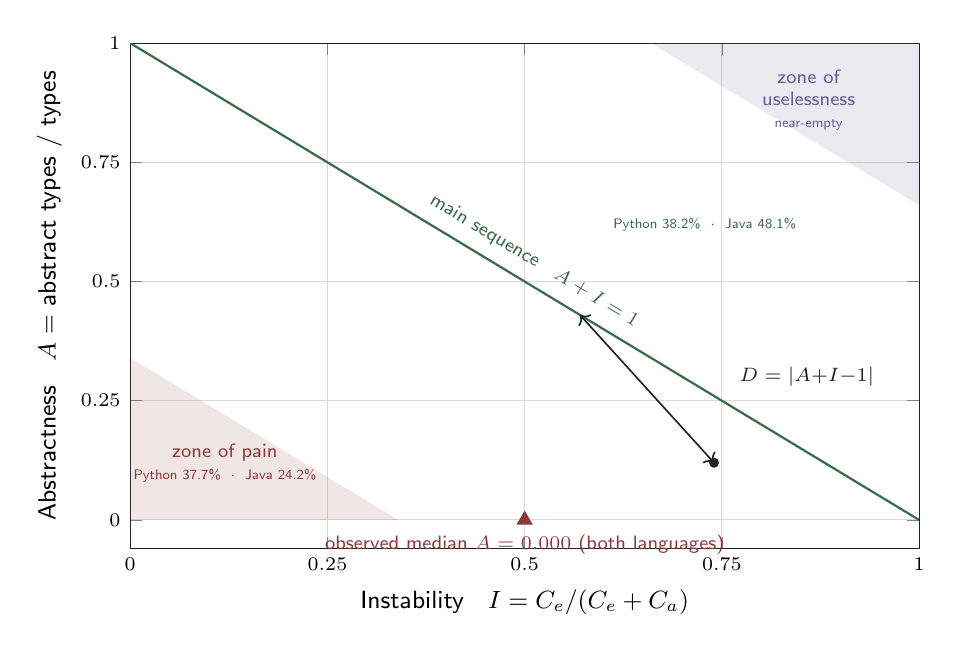
\begin{tikzpicture}
\begin{axis}[
  width=11.6cm, height=8.0cm,
  xlabel={Instability \; $I = C_e / (C_e + C_a)$},
  ylabel={Abstractness \; $A = $ abstract types $/$ types},
  xmin=0, xmax=1, ymin=-0.06, ymax=1,
  xtick={0,0.25,0.5,0.75,1}, ytick={0,0.25,0.5,0.75,1},
  axis line style={vbInk}, tick label style={font=\sffamily\scriptsize},
  label style={font=\sffamily\small},
  grid=major, grid style={draw=vbNote!25},
  clip mode=individual,
]
% zone of pain
\addplot[draw=none, fill=vbDrop, fill opacity=0.13]
  coordinates {(0,0) (0.34,0) (0,0.34)} \closedcycle;
\node[font=\sffamily\scriptsize, text=vbDrop, align=center]
  at (axis cs:0.12,0.12) {zone of pain\\{\tiny Python 37.7\% \;$\cdot$\; Java 24.2\%}};

% zone of uselessness
\addplot[draw=none, fill=vbStore, fill opacity=0.13]
  coordinates {(1,1) (0.66,1) (1,0.66)} \closedcycle;
\node[font=\sffamily\scriptsize, text=vbStore, align=center]
  at (axis cs:0.86,0.88) {zone of\\uselessness\\{\tiny near-empty}};

% main sequence
\addplot[thick, vbGood, domain=0:1, samples=2] {1-x};
\node[font=\sffamily\scriptsize, text=vbGood, rotate=-31, anchor=south]
  at (axis cs:0.50,0.51) {main sequence \; $A + I = 1$};
\node[font=\sffamily\scriptsize, text=vbGood, anchor=west]
  at (axis cs:0.60,0.62) {{\tiny Python 38.2\% \;$\cdot$\; Java 48.1\%}};

% D as distance -- label placed clear of the arrow
\addplot[only marks, mark=*, mark size=1.6pt, vbInk] coordinates {(0.74,0.12)};
\draw[<->, semithick, vbInk]
  (axis cs:0.74,0.12) -- (axis cs:0.57,0.43);
\node[font=\sffamily\scriptsize, text=vbInk, anchor=west]
  at (axis cs:0.76,0.30) {$D=|A{+}I{-}1|$};

% observed median, kept inside the axis box
\addplot[only marks, mark=triangle*, mark size=3pt, vbDrop]
  coordinates {(0.5,0.0)};
\node[font=\sffamily\scriptsize, text=vbDrop, anchor=north]
  at (axis cs:0.5,-0.012) {observed median $A = 0.000$ (both languages)};
\end{axis}
\end{tikzpicture}
\caption{\textbf{Package position, after Martin.} A package that is concrete and heavily
depended upon (bottom left) is painful to change; one that is abstract and depended upon by
nothing (top right) is dead weight. $D$ measures distance from the balanced diagonal. The
median package abstractness in this corpus is \textbf{0.000} in both languages --- half of all
packages contain no abstract type at all, which is the strongest package-level statement the
data supports. Position is reported as a descriptor only: $48.2\%$ of Python packages are
unplaceable because they contain no classes, against $5.7\%$ in Java, so the measurement has a
precondition that one language frequently fails to meet.}
\end{figure}

\clearpage

% =====================================================================
\section*{14. Validation protocol}
% =====================================================================

\begin{figure}[h]
\centering
\fitpic{%
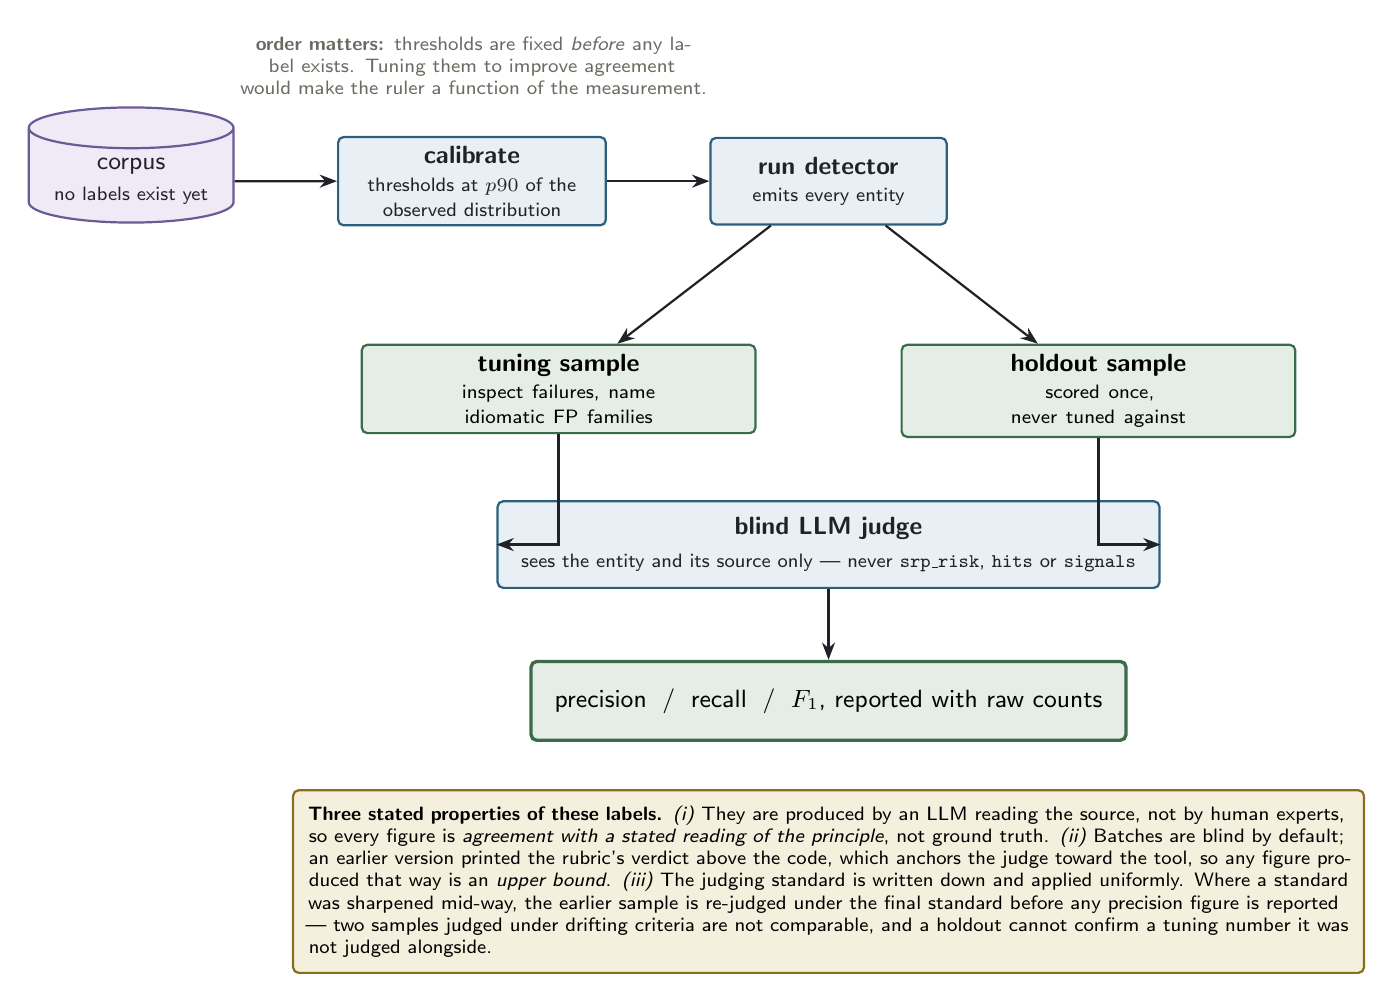
\begin{tikzpicture}[node distance=8mm]

\node[store, minimum width=26mm] (corpus) {corpus\\{\scriptsize no labels exist yet}};
\node[stage, right=13mm of corpus, minimum width=34mm] (calib)
  {\textbf{calibrate}\\[-1pt]{\scriptsize thresholds at $p90$ of the}\\[-2pt]{\scriptsize observed distribution}};
\node[stage, right=13mm of calib, minimum width=30mm] (run)
  {\textbf{run detector}\\[-1pt]{\scriptsize emits every entity}};

\draw[flow] (corpus) -- (calib);
\draw[flow] (calib) -- (run);

\node[note, above=4mm of calib, anchor=south, text width=68mm, align=center]
  {\textbf{order matters:} thresholds are fixed \emph{before} any label exists.
   Tuning them to improve agreement would make the ruler a function of the measurement.};

\node[keep, below left=15mm and -6mm of run, text width=44mm] (tune)
  {\textbf{tuning sample}\\[-1pt]{\scriptsize inspect failures, name}\\[-2pt]{\scriptsize idiomatic FP families}};
\node[keep, below right=15mm and -6mm of run, text width=44mm] (hold)
  {\textbf{holdout sample}\\[-1pt]{\scriptsize scored once,}\\[-2pt]{\scriptsize never tuned against}};
\draw[flow] (run) -- (tune);
\draw[flow] (run) -- (hold);

\node[stage, below=14mm of $(tune)!0.5!(hold)$, minimum width=72mm] (judge)
  {\textbf{blind LLM judge}\\[1pt]
   {\scriptsize sees the entity and its source only --- never \texttt{srp\_risk},
    \texttt{hits} or \texttt{signals}}};
\draw[flow] (tune) |- (judge.west);
\draw[flow] (hold) |- (judge.east);

\node[keep, below=9mm of judge, minimum width=72mm, draw=vbGood, very thick] (pr2)
  {precision \;/\; recall \;/\; $F_1$, reported with raw counts};
\draw[flow] (judge) -- (pr2);

\node[warn, below=6mm of pr2, anchor=north, text width=132mm]
  {\textbf{Three stated properties of these labels.}
   \emph{(i)} They are produced by an LLM reading the source, not by human experts, so every
   figure is \emph{agreement with a stated reading of the principle}, not ground truth.
   \emph{(ii)} Batches are blind by default; an earlier version printed the rubric's verdict
   above the code, which anchors the judge toward the tool, so any figure produced that way is
   an \emph{upper bound}.
   \emph{(iii)} The judging standard is written down and applied uniformly. Where a standard
   was sharpened mid-way, the earlier sample is re-judged under the final standard before any
   precision figure is reported --- two samples judged under drifting criteria are not
   comparable, and a holdout cannot confirm a tuning number it was not judged alongside.};

\end{tikzpicture}}
\caption{\textbf{Validation protocol.} Two structural properties defend against circularity:
thresholds are derived from the corpus distribution before labelling begins, and the judge
never sees the tool's own verdict. The holdout is scored once --- once it has informed a design
decision it is spent, and a further change requires a fresh sample.}
\end{figure}

\vspace{4mm}
\noindent\textbf{Figure sources.} All counts are from the 2026-08 run on
\texttt{AIDev-7.6M} (snapshot cutoff 2026-03-31): 1\,464 analyzable Python pull requests
across 484 repositories and 13\,310 source files, drawn from three agents at a 500-PR cap.
Validation figures are reported separately per principle and are not pooled across principles,
since the detectors differ in both unit of analysis and precision.

\end{document}
